\section{Introduction}
The detection of Gravitational Waves (GW) from compact binary coalescences (CBC) has been possible thanks to the joint effort of a number of different fields of expertise, all joining together to achieve the sophisticated detection process. GW data analysis concerns the detection of a GW signal hidden in the raw detector output (\textit{matched filtering}) and subsequently the inference of its physical properties (\textit{parameter estimation}). In order to accomplish its goal, GW data analysis relies on the availability of waveform (WF) templates to compare with the detector output.
To accurately explore the posterior distribution for the parameters defining a CBC, state-of-the-art parameter estimation (PE) algorithms~\cite{Aasi:2013jjl}~\cite{Veitch2014wba} can require the generation of as many as $10^7$ waveform templates. It is therefore paramount for the waveform generation to be as fast as possible. At the same time, because of the extreme sensitivity to phase differences in the likelihood  function, the templates must retain a high degree of accuracy to avoid biases in the posterior exploration.

\an{May be one should start with NR vs analytical models}

Many efforts have been devoted to solve Einstein equations for two coalescing objects and to predict the gravitational radiation emitted~\cite{}.
As solving the full equations is still extremely computationally challenging, the LIGO-Virgo Collaboration relies on approximate analytical models. 
These can be broadly categorized in  two families; (i) the effective-one-body(EOB) waveform 
models~\cite{Damour1999EOB}~\cite{Damour2009EOB}; (ii) the phenomenological models~\cite{}. 
EOB models are the analytically most complete family of analytical models available. 
They compute the GW signal by solving Hamilton's equations and accurately predict the GW signal up to late plunge.
The merger and ringdown  parts of the signal are then joint to the inspiral signal using information obtained from numerical relativity. 
Because of the numerical integrations involved, they tend to be accurate, but slow to generate, see however \cite{} 
for a much faster approach \sschmidt{(Is this about ROMs?? Or other??)}. 

The phenomenological waveform are based on the post-Newtonian formalism and then calibrated on EOB waveforms and numerical relativity. 
They tend to be faster than EOB models, but not as accurate.
Many efforts have been devoted to the task of speeding up the generation of GW signals from EOB families.
For example, one lead to the development of \textit{surrogate models}. Surrogate models are constructed 
starting from some decomposition in the waveform space followed by efficient interpolation to avoid any  numerical integration. 
Being fast to generate, they are routinely employed in GW data analysis. 
\par
A Machine Learning model is a promising alternative to the state-of-the-art waveforms generators. Machine Learning (ML) is a branch 
of statistics that is devoted to reproduce patterns read from data. A ML algorithm needs very little human input and, by a automatically solving an optimization problem, it is able to choose the best performing element among a large class of parametric models for the solution. This is the so-called training procedure. 
The ML flexibility in modeling data and reproducing trends is appealing: with a proper model choice and with an appropriate training 
procedure, we can hope to have a reliable, fast to execute generator of GW waveforms, while retaining the accuracy necessary for robust parameter estimation.
ML procedures have been applied so far to Numerical Relativity waveform data~\cite{Gabbard:2017lja,George:2017pmj,George:2017vlv,Rebei:2018lzh,Khan:2020foe}.
The construction of a NR-trained ML waveform model is currently missing except for a very restricted region of
the parameter space (nonspinning etc.). The main problem behind this is because of the need of a large set of
NR simulations that would be needed to train such an algorithm.

By contrast, an EOB model, informed by NR simulations, does not have such drawback as it can generate 
waveforms all over the BBH parameter space. However, since the dynamics and waveforms are analytically
incomplete, one has to rely on a certain amount of NR simulations to improve/complete the purely analytical
waveform through merger and ringdown. The NR information enters EOB models in two places: (i) on the one
hand, it allows to compute an accurate description of the merger and postmerger phase; (ii) on the other hand,
allows one to inform (or calibrate) some effective parameters entering the interacting Hamiltonian.
This is the case of the most recent avatar of the \texttt{TEOBResumS}~\cite{Nagar:2018zoe} model, 
\texttt{TEOBResumS\_SM}~\cite{Nagar:2020pcj}. This model used several hundreds (though many are redundant)
of availabe SXS simulations to compute a highly accurate description of the postmerger-ringdown phase
and just around 40 datasets to improve the behavior of the dynamics. The resulting model shows a 
mismatch, over Advanced LIGO noise, $\lesssim 4\times 10^{-3}$ all over $\sim 500$ hundred spin-aligned 
NR waveforms by the SXS collaboration. It is currently the most NR-faithful existing EOB model for spin-aligned 
binaries.
Thus we develop a ML waveform model for BBH coalescence that is trained by \texttt{TEOBResumS\_SM}.
Although higher modes are available in the original implementation, we focus here only on the dominant $\ell=m=2$
quadrupole waveform. We demonstrate that it can generate GW signals significantly faster than 
the original implementation, matching the performances of a Reduced Order Modelling 
(ROM)~\cite{Purrer_2014_ROM,Purrer_2016_FDROM,Boh2017SEOBNRv4}. 
At the same time it keeps the same accuracy of the underlying training model.
As a relevant physical application, we use the \texttt{TEOBResumS\_SMML} model to provide a completely new,
and independent analysis, of the 10 BBHs coalescence events collected in the O1/O2 LIGO-Virgo observing 
runs~\cite{LIGOScientific:2018mvr}. The physical parameters we find are compatible with previous
analyses obtained with radically different models~\cite{LIGOScientific:2018mvr}, though with some distinguo: 
(i) the individual masses obtained with our model are systematically {\it larger} than LVC published results; 
(ii) similarly, the individual spins of the objects, when measurable, are systematically larger than published
results. This is consistent with previously published analysis of GW150914 data using a slightly different version 
of \texttt{TEOBResumS}~\cite{Nagar:2018zoe}.


%Finally, our model can be employed for a systematic analysis of the detected signals so far. Being fast to run, it would perform accurate parameter estimation in a low amount of time and it could allow for a comparison between different surrogate WF models\footnote{Indeed it could be trained with different surrogate models: this would create a fast version of the underlying EOB model, which could be employed for parameter estimation.}
%, thus yielding invaluable information about the relevant physics.
On top of the specific application discussed here, our ML waveform model could also be used directly 
to speed up GW searches. Furthermore, since the time required to generate a WF does not depend
on the signal time length but only only on the number of grid points which the WF is evaluated at,
the applicability of our approach goes far beyond the LIGO/Virgo physics scenario. In particular,
we think about the forthcoming Einstein Telescope, that will be sensitive to very long stellar-mass 
inspirals from 5Hz, or to extreme mass ratio inspiral as LISA sources. In these context the problem
of WF fast generation will be more pressing and our approach, provided a suitable waveform model 
for training,  might be essential for detection and parameter estimation. 

The paper is organized as follows: 

%%%%%%%%%%%%%%%%%%%%%%%%%%%%%%%%%%%%%%%%%%%%%%
%\section{Problem specification}
\section{Conventions setup}
\label{sec:setup}
%--------------------------------------
A binary black hole is parametrized by a vector $ \boldsymbol{\vartheta} = (m_1,m_2, \mathbf{s}_1,\mathbf{s}_2) $, where $m_i$ are the BHs masses and $\mathbf{s}_i = \frac{\mathbf{S}_i}{m_i^2} <1$ are the \textit{dimensionless} spin. 
We call them the \textit{orbital parameters}.
Let the wave direction of propagation be identified with the spherical coordinates $(d_L, \iota, \varphi_0)$, where $d_L$ is the luminosity distance, $\iota$ the polar angle and $\varphi_0$ the azimuthal angle. The polar angle $\iota$ is also called inclination and it is measured with respect to the normal to the orbital plane.
A GW is parametrized as:
\begin{align} \label{eq:h_parametrization}
	&h(t, d_L,\iota,\varphi_0; \boldsymbol{\vartheta}) = h_+ + i h_\times \nonumber \\
		&\qquad= {\frac{\SI{1}{Mpc}}{d_L}} \sum_{l = 2}^{\infty} \sum_{m = -l}^{l} \tensor[^{-2}]{Y}{_{l m}}(\iota, \varphi_0) \cdot H_{lm}(t; \boldsymbol{\vartheta})
\end{align}
where $\tensor[^{-2}]{Y}{_{l m}}(\iota, \varphi_0)$ are the spin-2 spherical harmonics.
%In the expression, and for the rest of this paper, we included only the lowest order term in the multipole expansion, which is the dominant term in every realistic case.
We call $(m_1,m_2, \mathbf{s}_1,\mathbf{s}_2, d_L,\iota,\varphi_0)$ \textit{physical parameters} and they fully express the source 
proprieties as well as its orientation and position. In what follows, we will concentrate on the case in which 
spins $\mathbf{s}_1$ and $\mathbf{s}_2$ are \textit{aligned}. 

So, we approximate the full multipolar waveform with just the  the single complex quantity $H_{22}$ and we define
\begin{equation}\label{eq:h_std}
	\tilde{h}(t; \boldsymbol{\vartheta}) \equiv \tensor[^{-2}]{Y}{_{2 2}}(0,0) \cdot H_{22}(t; \boldsymbol{\vartheta}) = 4\cdot\sqrt{\frac{5}{64\pi}}H_{22}(t; \boldsymbol{\vartheta})
\end{equation}
and we express $\tilde{h}$ in terms of its amplitude and phase:
\begin{equation}\label{eq:h_ML}
	\tilde{h}(t; \boldsymbol{\vartheta}) = A(t; \boldsymbol{\vartheta}) e^{i \phi(t; \boldsymbol{\vartheta})} 
\end{equation}
%%%
We may also write $f_{\boldsymbol{\vartheta}}(t)$ to denote a function $f(t;\boldsymbol{\vartheta})$ of time with parametric dependence on $\boldsymbol{\vartheta}$.
In what follows, $f$ stands for any of the functions $A_{\tilde{\boldsymbol{\vartheta}}}(t)$ and ${\phi}_{\tilde{\boldsymbol{\vartheta}}}(t)$.
\par
With this definition, the full waveform can be expressed as:
\begin{align} 
	&h(t, d_L,\iota,\varphi_0; \boldsymbol{\vartheta}) =  \nonumber\\
		%&= {\frac{\SI{1}{Mpc}}{d_L}} \cdot \Bigg\{ \frac{1+\cos^2\iota}{2} \left[ \cos 2\varphi_0 \cdot \mathrm{Re}(\tilde{h}) 
		%	- \sin 2\varphi_0 \cdot \mathrm{Im}(\tilde{h}) \right] \nonumber \\
		%&+  i \cdot \cos\iota \left[ \sin 2\varphi_0 \cdot \mathrm{Re}(\tilde{h}) 
		%	+ \cos 2\varphi_0 \cdot \mathrm{Im}(\tilde{h})  \right] \Bigg\}
		&= {\frac{\SI{1}{Mpc}}{d_L}} \cdot \Bigg\{ \frac{1+\cos^2\iota}{2} \cdot A_{\boldsymbol{\vartheta}}(t)  \cos[\phi_{\boldsymbol{\vartheta}}(t)+2\varphi_0]  \nonumber \\
		&+ i \cdot \cos\iota \cdot A_{\boldsymbol{\vartheta}}(t) \sin[\phi_{\boldsymbol{\vartheta}}(t)+2\varphi_0] \Bigg\}
\label{eq:h_parametrization_simple}
\end{align}
where we split the real and the imaginary part of $h$ and we used the relation ${\tensor[^{-2}]{Y}{_{2 \pm 2}}(\iota, \varphi_0) = (1 \pm \cos \iota)^2 e^{\pm i 2 \varphi_0}}$.
We choose the convention that $\phi_{\boldsymbol{\vartheta}} = 0$ when the amplitude $A_{\boldsymbol{\vartheta}}$ has a maximum
\footnote{Indeed, a constant translation of $\phi_{\boldsymbol{\vartheta}}$ can be absorbed in the definition of $\varphi_0$ and does not affect the physics.}.
\par

%Aside from a numerical constant, the quantity ${\tilde{h}(t; \boldsymbol{\vartheta}) = A(t; \boldsymbol{\vartheta}) e^{i \phi(t; \boldsymbol{\vartheta})}}$ is the $h = h_+ +i h_\times$ strain, generated by a BBH with orbital parameters $\boldsymbol{\vartheta}$, when observed from the direction orthogonal to the total angular momentum ($\iota =0$), at a luminosity distance $d_L = \SI{1}{Mpc}$ and with $\varphi_0 =0$.
%$A(t)$ represent the amplitude of $\tilde{h}_+$ as a function of time, while $\phi(t)$ represent the phase of $\tilde{h}_+$ as a function of time.\footnote{
%We could have also worked with $\mathrm{Re}{\tilde{h}}$ and $\mathrm{Im}{\tilde{h}}$. However, such choice is most prone to numerical inaccuracies: the strain is a fast oscillating function and tracking its behavior is difficult.}
\an{All text above should be simplified!!}

%======================
\section{The model}
\label{sec: model}
%======================
%
The goal of the present work is to provide an accurate Machine Learning model which outputs the functions $A(t;\boldsymbol{\vartheta})$ and $\phi(t;\boldsymbol{\vartheta})$ (eq.~\eqref{eq:h_ML}), as generated by the state-of-the-art time domain WF models.
Because of scale invariance of GR, the dependence on total mass $M= m_1+m_2$ can be inserted analytically \cite{Arbey2019scaling} and we only need to consider the variables $\tilde{\boldsymbol{\vartheta}} = (q, s_1, s_2)$, where $q= m_1/m_2 \geq 1$.
More formally, we seek a ML model that reliably reproduces the following map:
\begin{align}
	(q, s_1, s_2) &\longmapsto A_{(q, s_1, s_2)}(t) \label{eq:objective_amp}\\
	(q, s_1, s_2) &\longmapsto \phi_{(q, s_1, s_2)}(t) \label{eq:objective_ph}
\end{align}
\sschmidt{Cited here the paper on scaling relations, beacause we used it and was really helpful. Keep it?}
\par
In the context of ML, our task reduces to performing two regressions\footnote{A regression is a statistical method to infer the relationship between a set of ``independent variables" and a set of ``dependent variable". A model consist in a functional form for such relation, usually with many free parameters to be specified. By looking at the data, one should be able to make a proper choice for their value.} 
from the orbital paramters to the amplitude and phase of WF. 
In order to be able to perform each regression, several steps are required.

\begin{enumerate}[label=(\Alph*)]
	\item \textit{Setting a time grid}. Each WF must be represented on a discrete time grid, which allows for efficient and reliable reconstruction on an arbitrary, user-given, grid. After this operation, the functions $A(t)$ and $\phi(t)$ are represented as vectors\footnote{
In ML jargon, this procedure is called preprocessing and aims to create a standard representation for all the data available (in our case the WFs).
}.
	\item \textit{Creating a dataset of WFs}. A large number of WFs must be generated on the the chosen time grid for a different number of orbital paramter $(q,s_1,s_2)$. This will be the training set for the ML model.
	\item \textit{Reducing the dimensionality of a WF}. In order to make a feasible regression, we need to reduce the dimensionality of a WF: we must be able to represent a single WF with very few real numbers. This operation must be invertible: once a low dimensional representation is given, one should be able to reconstruct the higher dimensional WF.
	\item \textit{Learning a regression}. Eventually, we train a model to perform the regression from $(q, s_1, s_2)$ to the low dimensional representation of the WF.
\end{enumerate}


\begin{figure}[!t]
	\centering
	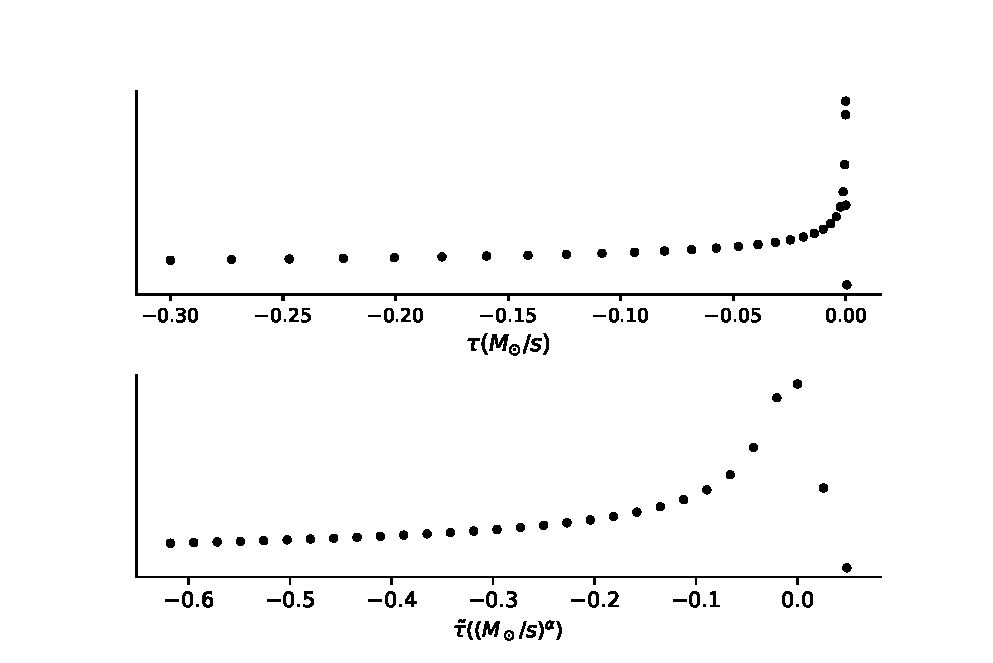
\includegraphics[width=\columnwidth,keepaspectratio]{tau_grid}
	\caption{Amplitude (arbitrary units) of a GW wave represented on a grid with 30 points.
It is set $\alpha = 0.3$ and $\tau_{min} = \SI{0.3}{s/M_\odot}$
The $\boldsymbol{\tau}$ grid is finer around the merger.
\sschmidt{Do we really need this??}
}
	\label{fig:tau_grid}
\end{figure}
%
\subsection{The time grid}
Each function $f$ to fit (i.e. amplitude and phase) must be represented by its values $\mathbf{f} \in \R^D$ on a discrete grid of $D$ points $\mathbf{t} \in \R^D$.
It is convenient to work in a grid of (dimensionless) reduced time $\boldsymbol{\tau} = \frac{\mathbf{t}}{M}$.
The time grid is chosen with the convention that at $\tau=0$ the function $A(t;\boldsymbol{\vartheta})$ (i.e. the amplitude of the $H_{22}$ mode) has a peak.
Once a time grid is set, the vector $\mathbf{f}$ is defined as follows:
\begin{equation}
	\mathbf{f}({\tilde{\boldsymbol{\vartheta}}})_i = f_{{\tilde{\boldsymbol{\vartheta}}}}(\boldsymbol{\tau}_i) \;\;\; 
\end{equation}
\par
The value of $f$ at an arbitrary time must be found by interpolation and this introduces an error in the reconstructed value.
To make the interpolation effective, we want a finer grid when the function changes much.
Clearly an equally spaced grid over times is not the best choice since the amplitude has a very narrow peak at $\tau=0$\footnote{As the phase has a rather regular behavior, it is not important to choose the right grid. For this reason a single grid for amplitude and phase, tuned on the behavior of amplitude, is used.}.
A good solution is to create an equally spaced grid $\boldsymbol{\tilde{\tau}}$ for the variable
\begin{equation} \label{eq:tau_tilde}
	{\tilde{\tau}} \equiv \sign{\tau} \cdot (|\tau|)^\alpha ;\;\; \alpha < 1
\end{equation}
and build the $\tau$ grid ${\boldsymbol{\tau}}$ as:
\begin{equation} \label{eq:tau_grid}
	{\boldsymbol{\tau}}_i = \sign{\boldsymbol{\tilde{\tau}}_i} \cdot (|\boldsymbol{\tilde{\tau}}_i|)^{\frac{1}{\alpha}}
\end{equation}
We call $\alpha$ \textit{distortion parameter}.
As can be seen in fig.~\ref{fig:tau_grid}, such choice ensures that more points are accumulated around the peak of amplitude.
\par
The lenght of the time grid determines the maximum lenght of the WFs that the model can generate.
Let us define $\tau_{min} = -{\boldsymbol{\tau}}_0 > 0 $ the starting point of the grid; this means that each WF start at a time $\tau_{min}\cdot M$ before the merger.
Note that $\tau_{min}$ is an important hyperparameter, set by the user, which strongly impacts on the model applicability.
\par
We find that the minimum frequency in the signal as a function of $M, q$ and $\tau_{min}$ is given by:
\begin{align}\label{eq:f_min}
	f_{min} = \SI{151}{Hz}  \left( \frac{(1+q)^2}{q} \right)^{\frac{3}{8}}  \left( \frac{M_\odot}{M} \right)  \left(\frac{\SI{1}{ \frac{s}{M_\odot}}}{\tau_{min}} \right)^{\frac{3}{8}}  
\end{align} 
The expression is approximate because it is obtained within a Newtonian framework and does not consider spin effects.
Nevertheless, it gives an useful estimation of the range of the applicability of the model.

\subsection{Dataset creation}
As in any ML method, we must create a dataset in order to perform training.
For our model, the dataset ${X \in \mathbf{Mat}(N,3+2D)}$ of $N$ waveform has the following form:
\begin{equation} \label{eq:dataset}
	X_{i:} = [q,s_1,s_2, {A}_{{\tilde{\boldsymbol{\vartheta}}}}^T, \boldsymbol{\phi}_{{\tilde{\boldsymbol{\vartheta}}}}^T]
\end{equation}
where $X_{i:}$ denotes the i-th row of the dataset matrix.
\par
The dataset is filled with random values of parameters ${\tilde{\boldsymbol{\vartheta}}}_i \sim \textrm{Unif}(\mathcal{P})$
\footnote{We denote by $\textrm{Unif}(\mathcal{P})$ a uniform probability distribution on the set $\mathcal{P}$.}.
To generate the training waves the \texttt{TEOBResumS} model is used.
Waves in eq.~\eqref{eq:h_std} are generated with a standard total mass $M = \SI{20}{M_\odot}$.
The output of the training model must be interpolated to the chosen time grid.
\par
It is important to ensure that all waves have zero phase at a constant time point $\bar{t}$: this is crucial to obtain a continuous dependence of the phase components on the orbital parameters. Model performances are not seen to depend on the choice of $\bar{t}$.
%%%%%%%%%%%%%
\subsection{Dimensionality reduction}
Once we are able to represent waveforms, a regressions ${\tilde{\boldsymbol{\vartheta}}} \longmapsto \boldsymbol{A}_{{\tilde{\boldsymbol{\vartheta}}}}, \boldsymbol{\phi}_{{\tilde{\boldsymbol{\vartheta}}}}$ is unfeasible. The dimension of the target space is too large for this task. Luckily, the elements of $\boldsymbol{A}, \boldsymbol{\phi}$ are strongly correlated with each other: the independent amount of information, required to fully reconstruct the wave, can be stored in a low dimensional vector.
A number of ML techniques to perform such a task are available. Among them, Principal Component Analysis (PCA) \cite[ch. 12]{murphy2012machine} was found to be particularly effective.
\par
The basic idea behind PCA is to seek a \textit{linear relation} between high dimensional and low dimensional data: high dimensional data ($\in \R^D$) are projected onto a $K$ dimensional subspace, by means of an orthogonal projection.
A theorem guarantees that, for zero mean data, the generators of subspace are the (orthonormal) first $K$ eigenvectors of the empirical covariance matrix $\Sigma \in \mathbf{Mat}(D,D)$. The eigenvectors are also called Principal Components (PCs) of the data.
Thus, the projection matrix $H\in \mathbf{Mat}(K,D)$ holds in each row the PCs and each high-dimensional point can be effectively expressed as a linear combination of the $K$ PCs\footnote{For this reason, PCA can also be seen as a perturbative expansion of a high dimensional observation. A more realiable reconstruction can be achieved by adding more and more PCs, each of which is less important than its previous.}.
\par
A PCA model is trained with the dataset eq.~\eqref{eq:dataset}: it represents an (approximate) bijective map between the high dimensional WF $\mathbf{f} = \boldsymbol{A}_{\tilde{\boldsymbol{\vartheta}}}, \boldsymbol{\phi}_{\tilde{\boldsymbol{\vartheta}}} \in \R^D$ and the low-dimensional representation $\mathbf{g} = \mathbf{g}_A , \mathbf{g}_\phi \in \R^K$.
%In what follows, $\mathbf{g}$ will be the PCA reduced lower order representation of $\mathbf{f}$ (i.e. of amplitude and phase).
The relation takes the following form:
\begin{align}
	\mathbf{g} = H (\mathbf{f} - \boldsymbol{\mu}) \label{eq:PCA_reduction_model}\\
	\mathbf{f} = H^T \mathbf{g} + \boldsymbol{\mu} \label{eq:PCA_reconstruction_model}
\end{align}
where $\boldsymbol{\mu}$ is the empirical mean vector ${\boldsymbol{\mu} = \frac{1}{N} \sum_{i=1}^N \boldsymbol{f}_i \in \R^D}$ and the matrix $H$ is computed from the empirical covariance ${\Sigma = \frac{1}{N} \sum_{i=1}^N (\mathbf{f}_i-\boldsymbol{\mu}) (\mathbf{f}-\boldsymbol{\mu})^T_i}$

%where, as usual in PCA, $H \in \mathbf{Mat}(K,D)$ is the matrix whose colums are the first K eigenvalues of the empirical covariance matrix $\Sigma = \frac{1}{N} \sum_{i=1}^N \mathbf{f}_i \mathbf{f}^T_i \in \mathbf{Mat}(D,D)$; the eigenvectors are also called principal components of the data (PCs). 
%In the equations above, the ${\tilde{\boldsymbol{\vartheta}}}$ dependence is omitted for notational simplicity.
\par

%%
\subsection{Regression}
Once a dimensional reduction (and reconstruction) scheme is available, the aim is to perform the regression
\begin{equation} \label{eq:regression_model}
	{\tilde{\boldsymbol{\vartheta}}} \longmapsto \boldsymbol{g}({\tilde{\boldsymbol{\vartheta}}})
\end{equation}
A number of ML models are avaiable for this purpose. The model Mixture of Experts (MoE) \cite{Jacobs1991AdaptiveMoE} \cite[ch. 11]{murphy2012machine} is found to be a good choice.
\par
MoE performs the following 1D regression:
\begin{equation} \label{eq:MoE}
	y(\mathbf{x}) = \sum_{l=1}^L (W^T \mathbf{x})_l \cdot \mathcal{S}(V^T\mathbf{x})_l
\end{equation}
where $\mathcal{S}$ is the \textit{softmax function}:
\begin{equation} \label{eq:softmax}
	\mathcal{S}(V^T{\mathbf{x}})_l = \frac{e^{(V^T{\mathbf{x}})_l}}{\sum_{l^\prime = 1}^L e^{(V^T{\mathbf{x}})_{l^\prime}}}
\end{equation}
and ${\mathbf{x}} \in \R^{\tilde{M}}$ and $V,W \in \mathbf{Mat}(\tilde{M},L)$.
The meaning of eq.~\eqref{eq:MoE} is clear: the output is a weighted combination of $L$ linear regressions $(W^T \mathbf{x})_l$ (called \textit{experts}); each expert perform a reliable regression in a small region of the space. The softmax function (in this context also called \textit{gating function}) switches on the expert contributions whenever this is required.
MoE is usually fitted with the Expectation Maximization (EM) algorithm, which iteratively sets the $W$ and $V$ by refining a lower bound to the log-likelihood of the model.
\par
Linear regression is a very simple model, often inadequate to model a complex relation. A simple trick to improve its performance is called \textit{basis functions expansion}. It consist in the replacement:
\begin{equation}
	{\mathbf{x}} \longrightarrow {\boldsymbol{\xi}}({\mathbf{x}}) = [\xi_1({\mathbf{x}}), \ldots, \xi_M({\mathbf{x}})]^T
\end{equation}
Thus, each expert becomes a non linear regression of the input ${\mathbf{x}}$.
A careful choice of basis functions can really make a difference in fit performances and it must be done at validation time, by comparing performances of different models.
\par
In our model, including in the $\xi_i$ every monomial up to 3/4th order in the three variables $ (\log q, s_1, s_2)$ is a good working choice
\footnote{
The choice of working with variable $\log q$ rather than $q$ gives much better validation results.
Heuristically, using $\log q$ prevents the values of the data features to vary too much within the range of interest, yielding more stable numerical performance.
}.
\par
The MoE is fitted with a reduced dimensional version of dataset~\eqref{eq:dataset}:
\begin{equation} \label{eq:dataset_MoE}
	G_{i:} = [q,s_1,s_2, \mathbf{g}_{A}(\tilde{\boldsymbol{\vartheta}})^T, \mathbf{g}_{\phi}(\tilde{\boldsymbol{\vartheta}})^T]
\end{equation}
The user must choose the number $L$ of experts to use and the basis functions features ${\boldsymbol{\xi}}({\tilde{\boldsymbol{\vartheta}}}) \in \R^{M}$ to use.
\par
As MoE model deals with single dimensional outputs, a single independent regression must be performed for each component $g_k$ of $\mathbf{g} \in \R^K$
\footnote{This is not a great limitation, because, due to orthogonality of PCs, each $g_j$ is independent from the other: we do not miss correlation among different regressions.}.
In general, a regression will be a collection of MoE weights ${\{ W^{(k)}, V^{(k)} \in \mathbf{Mat}(M,L_k) \}_{k=0}^K}$, where index $k$ labels different regressions for each PC.

\subsection{Summary}
The model has the following explicit form:
\begin{align}
	& \textrm{model}: \mathcal{P} \subset \R^3 \rightarrow \R^K \rightarrow \R^D \nonumber\\
	& {\tilde{\boldsymbol{\vartheta}}}
	\longmapsto  \mathbf{g}({\tilde{\boldsymbol{\vartheta}}} ) = 
		\begin{pmatrix}
		\sum_{l=1}^{L_1} (W^{(1)\;T} \boldsymbol{\xi})_l \cdot \mathcal{S}(V^{(1)\;T}\boldsymbol{\xi})_l \\
		\vdots \\
		\sum_{l=1}^{L_K}  (W^{(K)\;T} \boldsymbol{\xi})_l \cdot \mathcal{S}(V^{(K)\;T}\boldsymbol{\xi})_l
		\end{pmatrix}
	\nonumber \\	
	& \qquad \qquad \qquad \longmapsto \mathbf{f}({\tilde{\boldsymbol{\vartheta}}} ) = H^T \mathbf{g}({\tilde{\boldsymbol{\vartheta}}} ) + \boldsymbol{\mu} \label{eq:model}
\end{align}
where ${\boldsymbol{\xi}}({\tilde{\boldsymbol{\vartheta}}}) \in \R^M $ are the chosen basis function for the regression and $\mathcal{S}(\cdot)_k$ is the \textit{softmax} function eq~\eqref{eq:softmax}.
Two relations of the same type must be fitted, one for the amplitude, the other for the phase.
\par
Once weights are set properly, the expression provides an estimation for the waveform $\tilde{h}$ in \eqref{eq:h_std}.
The fitted expression for  $\tilde{h}$ is evaluated at constant mass $M = \SI{20}{M_\odot}$; the dependence on total mass is inserted analytically.
The dependence on $(d_L, \iota, \varphi_0)$ is computed with eq.~\eqref{eq:h_parametrization_simple}.
We are thus able to obtain a complex waveform $h(t;m_1,m_2, s_1, s_2, d_L, \iota, \varphi_0)$ which reproduces closely a waveform from the training model.
The model can generate a waveform also outside the range of orbital parameters, without guarantee to provide a reliable result.
\par
%%%% Where do I put it??
A Python implementation of the model is released in the package \texttt{mlgw}, publicly available at \href{https://pypi.org/project/mlgw/}{pypi.org/project/mlgw/}. The user can install it with the command \texttt{pip install mlgw}. The package provides also the gradients $\frac{\partial h}{\partial \vartheta_i}$ of the waveform.

%%%%%%%%%%%%%%%%%%
\section{Model performance}
We now discuss some tests on our model. We first study how its performance depends on the choice of hyperparameters. Furthermore, we assess the model accuracy and its limitations.
Finally, we measure the speed up provided by our model as compared with standard EOB methods.
As it is common, we measure the similarity between two waves by means of the \textit{optimal mismatch}:
\begin{align}
	\bar{\mathcal{F}}[h_1,h_2] &\equiv \min_{\phi_0} \left[ 1- \frac{\langle h_1, h_2 e^{i\phi_0} \rangle}{\sqrt{\langle h_1, h_1 \rangle \langle h_2, h_2 \rangle}} \right]	\label{eq:mismatch_def}
%\\
%	& = \min_{\phi_0} \left[ 1- \frac{ \mathrm{Re} \int \d{f} \; \frac{\tilde{A}_1 \tilde{A}_2}{S_n} e^{i(\phi_1-\phi_2-\phi_0)}}
%		{\sqrt{\left(\mathrm{Re} \int \d{f} \; \frac{\tilde{A}_1^2}{S_n}\right)
%		\left( \mathrm{Re} \int \d{f} \; \frac{\tilde{A}_2^2}{S_n} \right)}} \right] \nonumber
\end{align}
and we always use a flat noise curve (i.e. constant power spectral density for the detector noise).
%%%%%%%
\subsection{Validation}
Wherever relevant, we will employ a dataset with $5800$ waveforms generated in the domain $\mathcal{P} = [1,20]\times[-0.8,0.95]\times[-0.8,0.95]$, with $\tau_{min} = \SI{1.0}{s/M_\odot}$. The dataset was generated with TEOBResumS model \cite{}.
\paragraph{Dataset generation parameters}
We first evaluate the impact of number of grid points $N_{grid}$ and distortion parameter $\alpha$.
Let $\mathbf{f}_{N_{grid}, \alpha}$ the wave stored in a dataset where $\tau_{min}$ and $\mathcal{P}$ are fixed as above. We compare it with the output of the EOB model $\mathbf{f}_{EOB}$.
To compare the two waves, $\mathbf{f}_{N_{grid}, \alpha}$ must be evaluated on the dense time grid of EOB, by means of linear interpolation.
We then vary $N_{grid}$ and $\alpha$ and compute the resulting mismatch $\mathcal{F}[\mathbf{f}_{EOB}, \mathbf{f}_{N_{grid}, \alpha}]$.
We report the results in figure \ref{fig:N_grid}.
%%
\begin{figure}[!t]
	\centering
	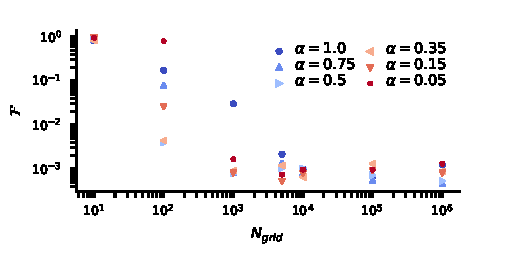
\includegraphics[width=\linewidth,keepaspectratio]{N_grid}
	\caption{Mismatch between waves $\mathbf{f}_{N_{grid}, \alpha}$ and raw waves from EOB model, as a function of time grid size $N_{grid}$. Each series refers to a different values of $\alpha$.
Mismatch is computed on $10$ test waves.  textwidth: \printinunitsof{in}\prntlen{\linewidth}
%The raw wave from EOB is evaluated at the original time grid provided by EOB: this means that it spans $\sim \SI{4}{s}$ sampled at $10^5$ step per second.
}
	\label{fig:N_grid}
\end{figure}
\par
As expected, we note that, by increasing the number of grid points, the mismatch decreases. Furthermore, using more than $\sim 10^3$ grid points, does not bring any improvement to mismatch. The result is dominated by numerical errors in the interpolations and it provides a lower-bound for the performances of the fit.
We note that a dataset grid with $\alpha\simeq 	0.35-0.5$ is a good choice.
It is effective if $N_{grid}$ does not grow too much. For a high number of grid points, different values of $\alpha$ yield almost equivalent results.
A good setting for dataset hyperparameters could be: $N_{grid} \simeq 2/3 \cdot 10^{3}$ and $\alpha \simeq 0.3/0.5$.
%%%%
\begin{figure}[!t]
	\centering
    \begin{minipage}{.5\linewidth}
        \centering
        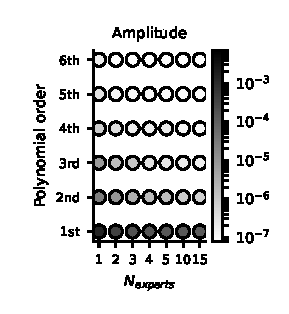
\includegraphics[width=\linewidth]{MoE_mismatch_amp}
    \end{minipage}\hfill
    \begin{minipage}{.5\linewidth}
        \centering
        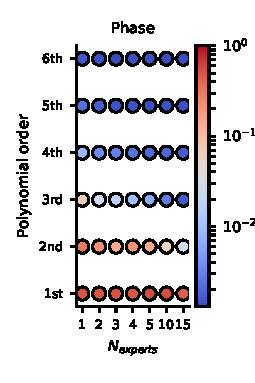
\includegraphics[width=\linewidth]{MoE_mismatch_ph}
    \end{minipage}
	\caption{Validation results for fit of MoE model. Each point corresponds to a MoE regressions for the amplitude (left) and phase (right), with a different values of expert number $N_{exp}$ and order of polynomial basis function.
The amplitude and phase are represented with 5 and 4 PCs respectively.
In the colorbar, we represent the mismatch on test waves: it is obtained by reconstructing test waves with fitted amplitude (phase) and test phase (amplitude).
}
	\label{fig:MoE_test}
\end{figure}


\paragraph{MoE parameters}
In what follows, we will focus on setting a small number of hyperparameters relevant to MoE model: the number of experts $N_{exp}$ for each component model, the basis functions $\xi_i(\boldsymbol{\tilde{\vartheta}})$ to use in basis function expansion and the number $N_{train}$ of training points to use.
Other parameters, related to the details of the training procedure, will not be considered.
\par
In figure \ref{fig:MoE_test} we show our results.
We fitted a model for amplitude (or phase) for different configurations of expert number $N_{exp}$ and polynomial basis function.
By label "n-th order", we mean that in the basis function expansion, every monomial up to n-th order is used.
We report with a colorbar the value of the mismatch $F$ between test and reconstructed WFs. The MoE models for each component share the same number of experts $N_{exp}$.
The test mismatch for the fitted amplitude (phase) is computed by using the test phase (amplitude) in the reconstructed wave.
\par
Interpretation of the results is straightforward. Fit performances improves, as the model complexity (i.e. number of fittable parameters) increases.
In general, we note that adding more features (i.e. improving expert's flexibility) is more effective than increasing the number of experts.
However, model performances do not improve indefinitely. As model complexity increases beyond a threshold, performance does not get any better.
Such threshold is around a model with 4 experts and 4th order polynomial regression. This "simple" model match the performances of much more complex models and thus it should be deemed as the best choice.
%%%%%%%%%
\begin{figure}[!t]
	\centering 
    \begin{minipage}{.5\linewidth}
		\centering
	    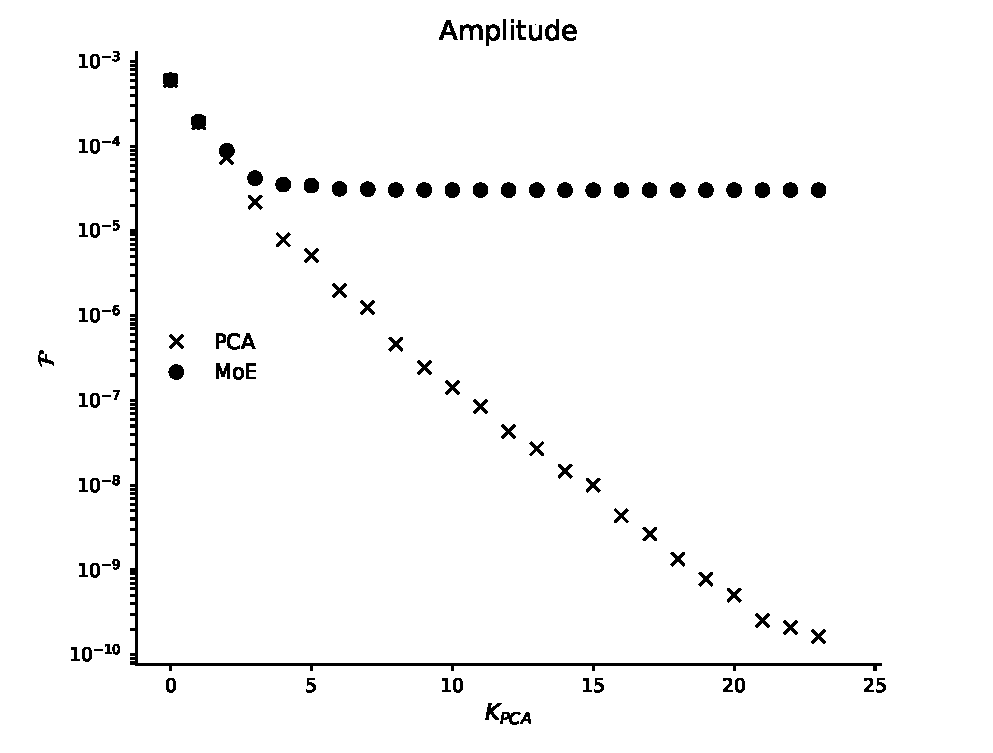
\includegraphics[width=\linewidth]{mismatch_MoE_vs_PCA_amp}
	\end{minipage}\hfill
    \begin{minipage}{.5\linewidth}
		\centering
	    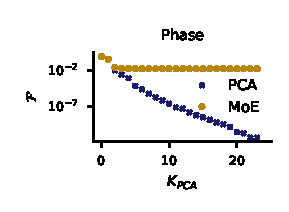
\includegraphics[width=\linewidth]{mismatch_MoE_vs_PCA_ph}
	\end{minipage}
	\caption{Test mismatch as a function of the number of PCs used in the low dimensional representation.
Label "PCA" refers to waves reconstructed with PCA only; points with label "MoE" are reconstructed after a MoE regression.
Data refers to amplitude (left panel) and phase (right panel).
MoE model is chosen to be the optimal one with $4$ experts and a fourth order polynomial.
}
	\label{fig:mismatch_MoE_vs_PCA}
\end{figure}
%%%%%%%%%
\paragraph{Choosing the number of PCs}
Of course, the accuracy of the reconstruction of the low dimensional representation depends on the number $K$ of principal components considered: the more PCs are used, the best accuracy can be achieved.
However in practice, due to error in the MoE regression, one cannot reduce the reconstruction mismatch arbitrarily and should not choose the number of PCs to fit before having seen the MoE accuracy.
At high PC order the relations to fit become noisy and the regression becomes less accurate, eventually washing out any improvement brought by a higher number of PCs.
\par
In figure \ref{fig:mismatch_MoE_vs_PCA} we report a numerical study of this. We plot the reconstruction mismatch as a function of the number of PCs considered. We consider separetely regression for the amplitude and for the phase. In one series, we reconstruct the wave using true values of PCs: the mismatch is a measure of PCA accuracy. In the other series, we reconstruct a wave using values for PCs as guessed by MoE regression: this is a measure of accuracy of both PCA and regression.
For the first two PCs, the regression is accurate enough for reproducing the PCA accuracy.
On the other hand, any regression beyond the 4th PCA component does not give any improvement to the MoE mismatch: the noise in the relation of high order PCs is too high for a regression to be performed.
\par
In the PCA, we include every PC which yields improvement in MoE mismatch. For our model, $K = 5(4)$ is a good choice for amplitude (phase).
Of course, this strongly depends on the regression model: the more precise the model is, the more PCs can be included.
However, any model cannot increase its accuracy indefinitely. Every surrogate model has an intrinsic noise level, due to numerical error and to the approximations in the physical model.
%%%%%%%%%%%%%
\paragraph{Choosing the number of training points}
The choice of the number of training points $N_{train}$ must trade between accuracy and speed of execution. Too many training points will make the training slow and unfeasible, while too few training points will yield a poor model, which does not generalize data (underfitting).
In the choice of number of training points, the comparison between train and test error will provide important information on how the model is able to generalize the trend.
\par
In figure \ref{fig:N_train} we report train and test value of mismatch and mse of first 3 PCs as a function of the number of training points. Data refers to a MoE model fitted for 4 PCs of the phase dataset. The models has ${N_{exp} = 4}$ and performs basis function expansion with a fourth degree polynomial. Test mismatch are obtained using test amplitude to reconstruct the waveform; this is not a great limitation as any error in phase reconstruction dominates the overall mismatch (see e.g. fig.~\ref{fig:mismatch_MoE_vs_PCA}).
\begin{figure}
	\centering
    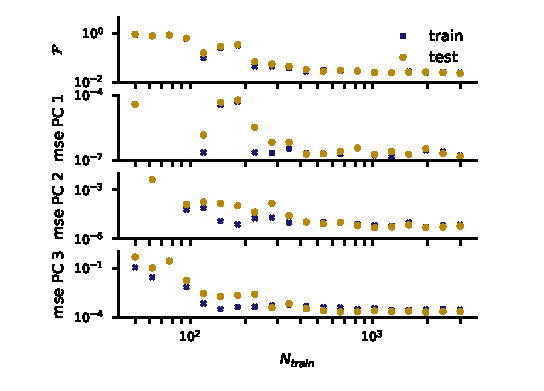
\includegraphics[width=\linewidth]{N_train}
	\caption{Train and test error for MoE fit of 4 PCs of phase, as a function of the number of training points. We report train and test reconstruction mismatch (top) and mse for the first 3 PCs (below).
    MoE model employs 4 experts and a fourth order polynomial for a basis function expansion.
    }
	\label{fig:N_train}
\end{figure}
\par
As $N_{train}$ increases, we see a steady decrease of the errors, until a plateau is reached.
We note that overfitting is not a problem. For a reasonably high number of training points ($N_{train} \gtrapprox 50$) train and test error are close to each other.
For $N_{train} \gtrapprox 800$, the trend stabilises and increasing training points does not affect much model performance.
In the present model, setting $N_{train} \simeq \SI{3000}{}$ is a good choice
\footnote{As compared with standard neural networks, which routinely employ $O(10^5)$ points datasets, this is an incredibly low amount of data. This is due to the fact that MoE is a simple model with a few number of parameters: few data are enough for learning a reliable relation.}.
%%%%%%%%%%%%%%%%%%%%%%
\subsection{Accuracy}
%%%%
\begin{figure}
	\centering
    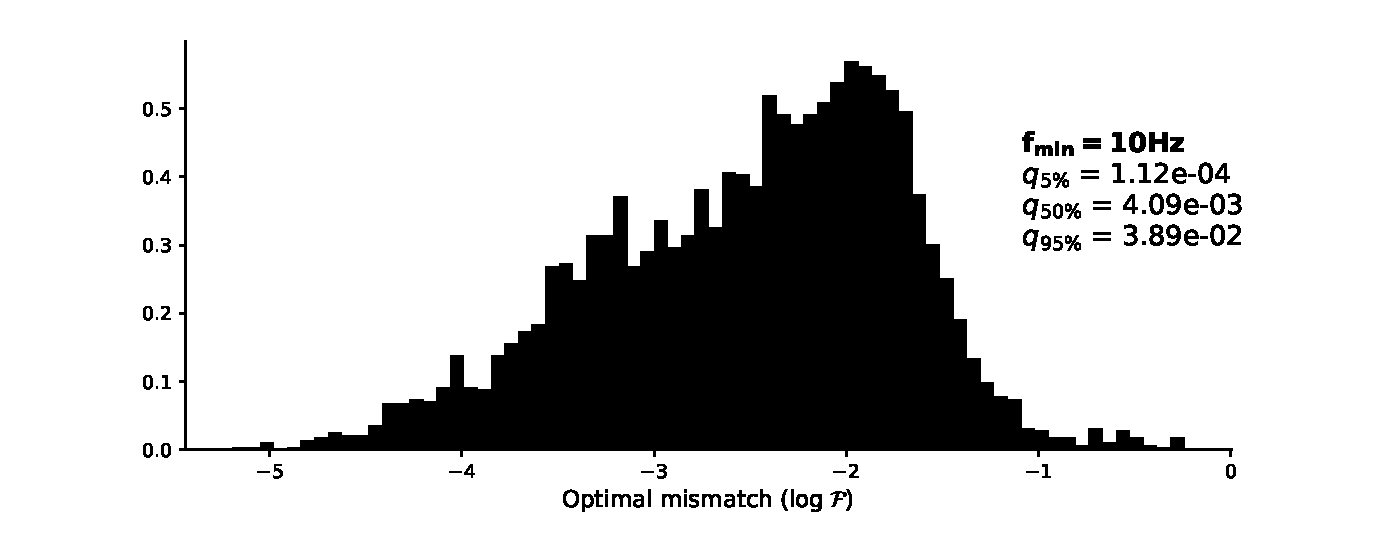
\includegraphics[width=\linewidth]{F_hist}
	\caption{Histogram for the logarithm of mismatch values, computed on $N=4000$ test waveforms. Each WF is generated with random orbital parameters $(m_1,m_2, s_1, s_2, d_L, \iota, \phi_0)$ and with a starting frequency of $\SI{10}{Hz}$.
We report the median value $q_{50\%}$ as well as the positions $q_{5\%}$ and $q_{95\%}$ of the 5th and 95th percentile.
The $95\%$ of the test waves have a mismatch lower than $7.5 \cdot 10^{-3}$.
}
	\label{fig:F_hist}
\end{figure}
%%%%
We compute mismatch value on a number of WFs with random values of the physical parameters (i.e. $m_1,m_2, s_1, s_2, d_L, \iota, \varphi_0$) for each wave.
We report our results in the histogram in figure~\ref{fig:F_hist}.
We report a median value of the distribution $\mathcal{F}_m = 4 \cdot {10^{-3}}^{+???}_{-???}$. Such results are similar to the discrepancies between state-of-the-art models.
\par
To understand better model performances, it is interesting to display the accuracy as a function of the orbital parameters $\boldsymbol{\vartheta} = (q,M,s_1,s_2)$.
We generate waves for randomly chosen values of $\vartheta = (q, M, s_1, s_2)$ and, for each wave, we measure test mismatch $\mathcal{F}$ and mse on the reconstruction of the first PC for the phase.
The latter is useful to test the accuracy of the fit before wave reconstruction.
The results are reported in the contour plots in figure \ref{fig:countour}.
\sschmidt{Probably the comments below are not really interesting...}
\par

%%
\afterpage{
\begin{figure}[!ht]
	\newcommand{\minipagesize}{.5}
	\newcommand{\titlefontsize}{7}
	\centering 
    \begin{minipage}{\linewidth}
        \centering
	 	\begin{minipage}{\minipagesize\linewidth}
		    \centering
			{\fontfamily{DejaVuSans-TLF} \fontsize{\titlefontsize}{12}\selectfont 
			Mismatch%
			} \\
			\vskip0.3em
		    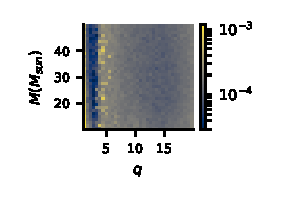
\includegraphics[width=\linewidth]{F_countour_mass}
		\end{minipage}\hfill
		\begin{minipage}{\minipagesize\linewidth}
		    \centering
			{\fontfamily{DejaVuSans-TLF} \fontsize{\titlefontsize}{12}\selectfont 
			Mean Squared Error%
			} \\
			\vskip0.3em
		    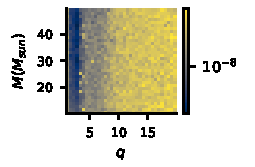
\includegraphics[width=\linewidth]{mse_countour_mass}
		\end{minipage}
    \end{minipage}\hfill
    \begin{minipage}{\linewidth}
        \centering
	 	\begin{minipage}{\minipagesize\linewidth}
		    \centering
		    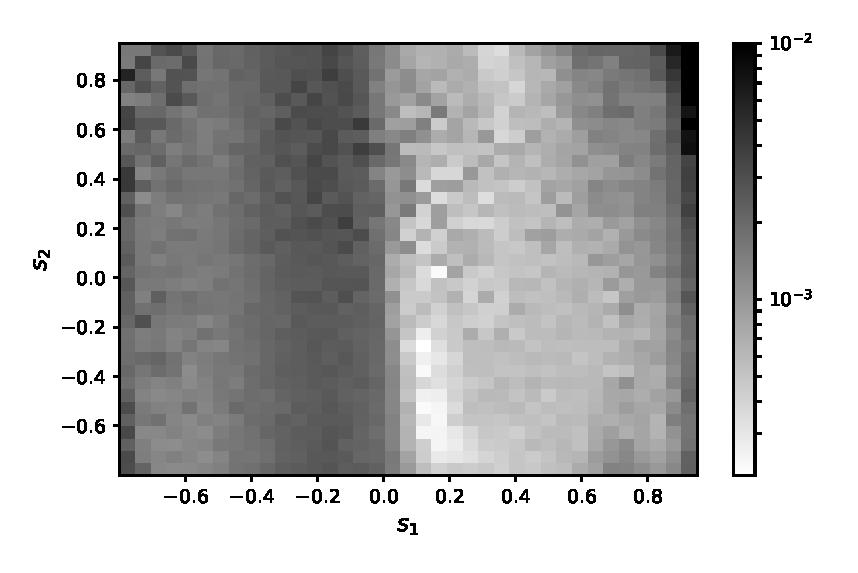
\includegraphics[width=\linewidth]{F_countour_spins}
		\end{minipage}\hfill
		\begin{minipage}{\minipagesize\linewidth}
		    \centering
		    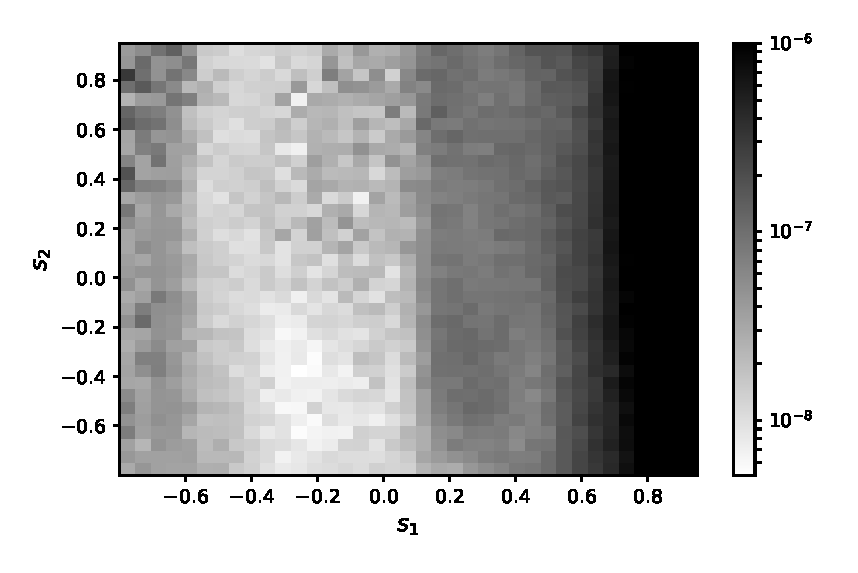
\includegraphics[width=\linewidth]{mse_countour_spins}
		\end{minipage}
    \end{minipage}\hfill
    \begin{minipage}{\linewidth}
        \centering
	 	\begin{minipage}{\minipagesize\linewidth}
		    \centering
		    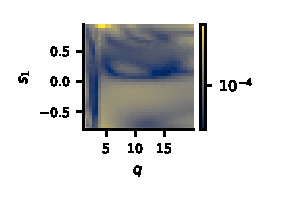
\includegraphics[width=\linewidth]{F_countour_q_s1}
		\end{minipage}\hfill
		\begin{minipage}{\minipagesize\linewidth}
		    \centering
		    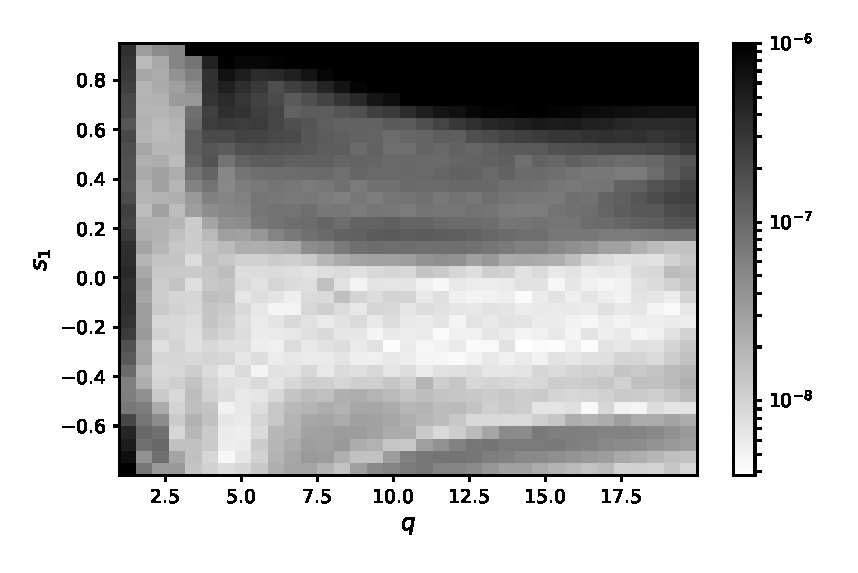
\includegraphics[width=\linewidth]{mse_countour_q_s1}
		\end{minipage}
    \end{minipage}
	\caption{We report test mismatch and mse for the first PC of the phase, as a function of the orbital parameters $\vartheta = (q, M, s_1, s_2)$. The histograms holds $145061$ waveforms, randomly drawn by varying the relevant parameters.
In the left column, the color mesh refers to test mismatch; in the right column, we report test mse.
On the x-y we display values of two physical quantities, each discretized in $35$ bins.
On top row, we display $q$ vs $M$ dependence. On central row, we present spins dependence ($s_1$ vs $s_2$). On bottom row, we show $q$ vs $s_1$ dependence.
Each wave starts $\SI{8}{s}$ before merger.
}
	\label{fig:countour}
\end{figure}
%\clearpage
}
%%%
\par
By looking at the top line of \ref{fig:countour}, we note that the mse does not depend on $M$. This was to be expected because the total mass dependence is inserted analytically within the model.
%However, we observe that, at constant $q$, at lower $M$ values, the mismatch is higher. This is explained on physical basis. In the Newtonian approximation $\phi(t) \sim M^{-5/8}$ for constant time to merger. Thus If $M$ is small, the value for phase is high: the two waves have more cycles to "accumulate mismatch".
\par
Again on the top line, we note that both $\mathcal{F}$ and mse depend (quite strongly) on $q$.
The mismatch and mse are well correlated: the reconstruction of the wave and the interpolation do not affect much the mismatch.
We note that for low values of $q$ the fit shows poor performance: in that region the relation to catch is less smooth, making the regression less reliable.
\par
In the center line of \ref{fig:countour}, we displayed the dependence on spins.
As long as the $s_1$ dependence is considered, the most striking feature is the inverse correlation of mismatch and mse for the first phase PC.
This means that the value of the first PC does not affect much the spin dependence of the waveform and that, being non-leading, spin contribution become important at lower order of PCs.
Indeed, the values of the first PC are well correlated with mismatch in the case of $q$. See~\cite{Ohme2013PCA_GW} for a closely related discussion on PCA components and its dependence on physical parameter.
\sschmidt{Is it fine to cite this? Is it relevant?}
\par
Apart from this feature, we note that the mismatch tends to grow for high spins: the fit is less reliable in such regions.
\par
In the third row of \ref{fig:countour}, we displayed the dependence on $q$ and $s_1$, the variables on which the error depends more.
We note again the inverse correlation between the mismatch and mse, when considering the $s_1$ dependence.
%%%%%%%%%%%%%%%%%%
%%%%%%%%%%%%%%%
\subsection{Runtime analysis} \label{sec:runtime}
We now asses the time performances of our model.
We are interested to make a comparison with both \texttt{TEOBResumS} (the train model and the state-of-the-art in accuracy) and \texttt{SEOBNRv4\_ROM} \cite{} (the state-of-the-art in speed of execution).
We then measure the time that our code takes to generate a WF.
\paragraph{Comparison with \texttt{TEOBResumS}}
When dealing with a real detection scenario, we are often interested in generating a WF which starts from a given frequency $f_{min}$, which is usually set by the detector's sensitivity window.Thus, it is crucial to measure the speed up that our model can provide in performing such task.
We define the speed up $\mathcal{S}$ as the ratio between the runtime of benchmark model and the runtime of \texttt{mlgw} to produce the a waveform starting from a given $f_{min}$. Each waveform is produced with constant total mass $M = 100 M_{\odot}$ and random parameters; the WF is sampled at $f_{sam} = \SI{2048}{Hz}$.
We consider the two cases with $f_{min} = \SI{5}{Hz}$ and $f_{min} = \SI{20}{Hz}$; the first choice refers to the hypotetical lower bound for the sentivity of the Einstein telescope (ET), while the second is close to that of Advanced-LIGO/Virgo.
In figure~\ref{fig:time_performance_hist} we report the histogram of the measured speed up values for model \texttt{TEOBResumS}.

\newcommand{\factor}{.9}
\begin{figure}
	\centering
	\begin{minipage}{\factor\linewidth}
	    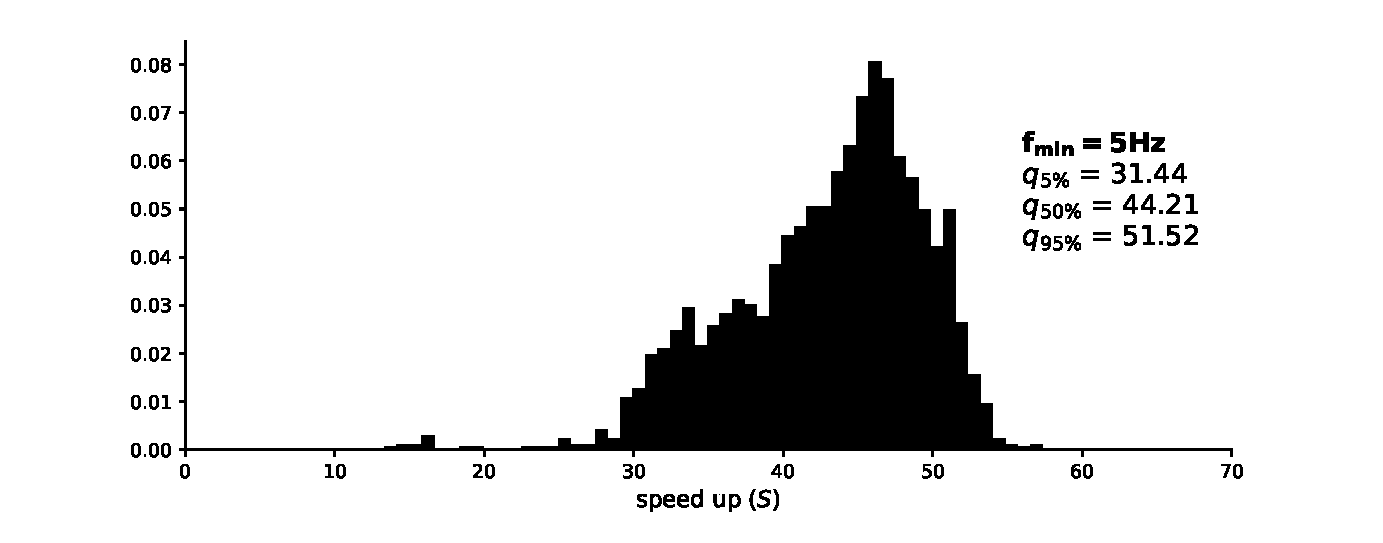
\includegraphics[width=\linewidth]{time_performance_hist_5}
	\end{minipage}\hfill
	\begin{minipage}{\factor\linewidth}
	    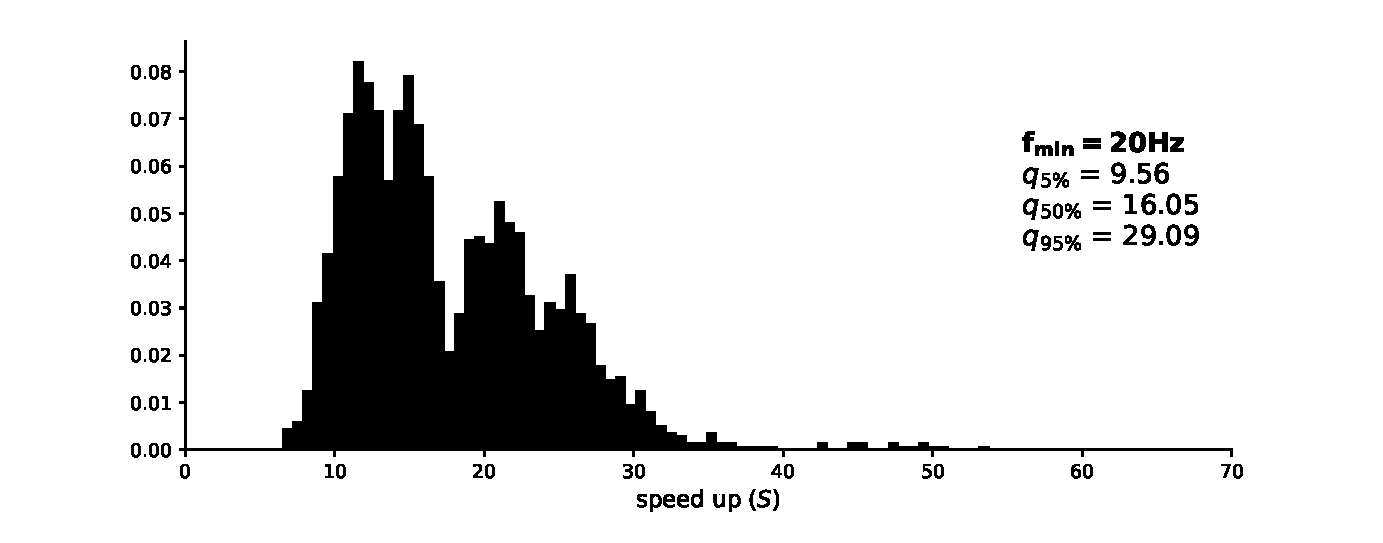
\includegraphics[width=\linewidth]{time_performance_hist_20}
	\end{minipage}

	\caption{
Histogram for values of the speed up given by \texttt{mlgw}, as compared with \texttt{TEOBResumS} model, computed on $N=2000$ test waveforms. Each WF is generated with random physical parameters and has a minimum frequency of $\SI{5}{Hz}$ (top panel) and $\SI{20}{Hz}$ (bottom panel).
We set a constant total mass $M=\SI{100}{M_\odot}$ and the sampling rate $f_{sam} = \SI{2048}{Hz}$.
We report the median value $q_{50\%}$ as well as the positions $q_{5\%}$ and $q_{95\%}$ of the 5th and 95th percentile.
\sschmidt{Are you really sure that two peaks are fine?? Understand this...}
}
	\label{fig:time_performance_hist}
\end{figure}
%%%%%%%%%%
\begin{figure}
	\centering
	\begin{minipage}{\factor\linewidth}
	    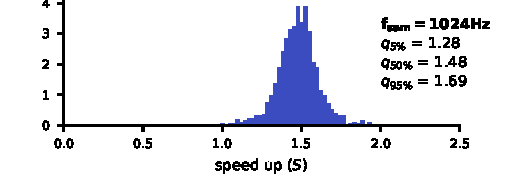
\includegraphics[width=\linewidth]{time_performance_hist_ROM_20_1024}
	\end{minipage}\hfill
	\begin{minipage}{\factor\linewidth}
	    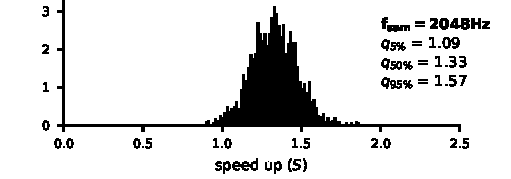
\includegraphics[width=\linewidth]{time_performance_hist_ROM_20_2048}
	\end{minipage}

	\caption{
Histograms for values of the speed up given by \texttt{mlgw}, as compared with ROM model \texttt{SEOBNRv4\_ROM}, computed on $N=2000$ test waveforms.
Each WF is generated with random physical parameters and has a sampling frequency $f_{sam}$ of $\SI{1024}{Hz}$ (top panel) and $\SI{2048}{Hz}$ (bottom panel).
We set a constant total mass $M=\SI{100}{M_\odot}$ and the same starting frequency $f_{min} = \SI{20}{Hz}$.
We report the median value $q_{50\%}$ as well as the positions $q_{5\%}$ and $q_{95\%}$ of the 5th and 95th percentile.
}
	\label{fig:time_performance_hist_ROM}
\end{figure}

%%%%%%%%%%
We see that in both cases a substantial speed up is achieved. The speed up is higher for longer WFs
\footnote{This is clearly understood: a longer WF requires more computation for a EOB model, while roughly the same amount of work is done by mlgw}, 
making our model particulary convenient for advanced detectors, with a larger sensitivity window.
\par
\paragraph{Comparison with \texttt{SEOBNRv4\_ROM}}
In figure~\ref{fig:time_performance_hist_ROM} we report the histogram of the measured speed up values for model \texttt{SEOBNRv4\_ROM}, which is now the state of the art for the WF generation time.
The comparison is made in the same wave as above only for the $f_{min} = \SI{20}{Hz}$; the ROM has not been built for $f_{min} = \SI{5}{Hz}$.
As the ROM model yields WFs in frequency domain, in the time comparison we included a fast Fourier trasform (FFT) of the time domain WF of \texttt{mlgw}. This is to ensure that we evaluate the two model at the same conditions.
Interestingly, the time taken by the FFT (in the numpy implementation) is similar to that required to generate a WF. Thus for a WF in FD our model cannot be substantially faster, due to the limitation imposed by the FFT.
\par
We note the the performances are quite similar to each other.
If a lower sampling rate is employed, \texttt{mlgw} slighly improves its performances.
\par
It is important to stress that \texttt{mlgw} is written in pure Python, while \texttt{SEOBNRv4\_ROM} is coded in C. Thus, the fact the the two models show similar performances is remarkable: surely, a C implementation of \texttt{mlgw} would be faster than \texttt{SEOBNRv4\_ROM}.
Furthermore, \texttt{mlgw} is more efficient in reconstructing the waveforms: it requires only $O(5\cdot 10^3)$ WFs for the training, while in order to build a ROM as many as $O(5\cdot 10^5)$ WFs are required.
\par
%%%
\paragraph{Profiling}
It is interesting to have a knowledge of the time spent by \texttt{mlgw} in each stage of the WF generation procedure.
We generate $100$ waves with random physical parameters and we measure the CPU time spent to execute each basic task.
In table \ref{tab:profiling}, we compare the results for two values of $N_{grid}$.
\begin{table}
	\def\arraystretch{1.5}
	\begin{tabular}{ l c c }
		\multirow{2}{*}{Task (for 100 WFs)}& \multicolumn{2}{c}{CPU time (ms)}\\
			&$N_{grid} = 10^3$	& $N_{grid} = 10^5$\\
	\hline \hline
		 Generation of raw WF 			& $6.9 \; (46.9\%)$	& $7 \; (1.6\%)$ \\ 
	\hline
		 Interpolation to the user grid & $4.5 \; (30.6\%)$	& $194 \; (45.3\%)$ \\ 
	\hline
		 Post processing 				& $1.7 \; (11.6\%)$	& $206 \; (48.1\%)$ \\
	\hline
		 Total							& $14.7 \; (100\%)$ &  $428 \; (100.0\%)$ \\
	\hline \hline
	\end{tabular}
	\caption{
Time taken by different stages of the generation of $100$ waveforms; data refers to two different values of $N_{grid}$.
Generation of raw WF refers to the computation of the strain $\tilde{h}$ as produced by a ML model. Interpolation to user grid evaluates the WF on the grid chosen by the user. In the post-processing phase, the dependence on $d_L$, $\iota$ and $\varphi_0$ is included.
}
	\label{tab:profiling}
\end{table}
\par
We see that the cost of generating the raw WF does not depend on the number of grid points. On the other hand, the interpolation and the post processing depends on $N_{grid}$ and their cost grows dramatically as the user requires more and more points.
It is important to stress that the latter two tasks are slow only because they deal with a huge amount of data. Indeed they perform trivial and ``quick" operations and their execution relies on well optimized \texttt{numpy} routines.
If such huge amount of datapoints is required, very little space is left for speed up.
\par

\section{Application to GWTC-1}

We test the implementation of our TEOBResumS model on the public data from GWTC-1, the first GW catalog~\cite{}. 
The GWTC-1 catalog consists of 10 BBH systems and a BNS system. Because of the training of the WF model, we do not analyse GW170817, the BNS system, and concentrate exclusively on the BBH signals. Our parameter estimation algorithm is \texttt{gwmodel}~\cite{} a publicly available infrastructure 
written in a mixture of \texttt{Python} and \texttt{cython} that serves as interface for the parallel nested sampling implementation \texttt{cpnest}~\cite{}. 
The analysis of each BBH system is set up as follows; we choose a total of 2000 Live Points, four parallel MCMC chains with a maximum length of 5000 steps to ensure that each successive sample is independent of the previous. These settings yield an average of $\sim$ 15000 posterior samples and 
evidence calculations that are accurate to the first decimal digit. For each BBH system we choose prior distributions as described in the GWTC-1 release paper~\cite{}. Finally, and critically, to ensure that our results can be compared fairly to published ones, we employ the power spectral densities released as part of GWTC-1. No calibration uncertainty model is assumed for these runs. 
\begin{figure}
	\centering
    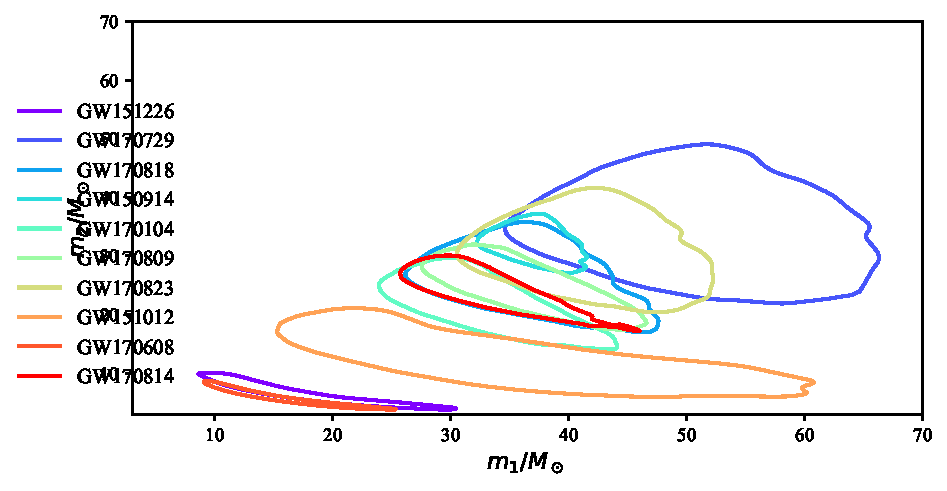
\includegraphics[width=.75\linewidth, trim = {3cm 0cm 3cm 0cm}]{img/posterior_masses_source.pdf}
	\caption{
Two-dimensional posterior distributions for the component masses for all BBH systems in GWTC-1.
}
	\label{fig:summary-masses}
\end{figure}

Figure~\ref{fig:summary-masses} and Table~\ref{tab:summary} summarise our results. In Table~\ref{tab:summary} we report exclusively 
summary statistic for the intrinsic parameters of the system. All mass parameters quoted are in the source frame. The redshift of each BBH is estimated 
from its luminosity distance posterior and converted into a redshift by assuming the cosmological parameters given in Ref.~\cite{}.

\begin{table}[]
\centering
\caption{Summary table for the inferred intrinsic parameters from MLGW and the released GWTC-1 credible intervals. All mass parameters quoted are computed in the source frame, see the text for details of the calculation. For GWTC-1 we report results from Table III, thus coming from averaging over two waveform models. The uncertainties correspond to the 90\% credible intervals.}
\label{tab:summary}
\begin{tabular}{cccccc|ccccc}
                              & \multicolumn{5}{c}{MLGW}                                                   & \multicolumn{5}{c|}{GWTC-1}                                                \\ \hline
\multicolumn{1}{c|}{Event}    & $m_1/M_\odot$ & $m_2/M_\odot$ & $\mathcal{M}/M_\odot$ & $q$ & $\chi_{eff}$ & $m_1/M_\odot$ & $m_2/M_\odot$ & $\mathcal{M}/M_\odot$ & $q$ & $\chi_{eff}$ \\ \hline
\multicolumn{1}{c|}{GW150914} & $36.4_{-2.6}^{+4.7}$& $32.6_{-4.4}^{+2.9}$& $32.8_{-1.5}^{+1.7}$& $0.9_-{0.2}^{+0.1}$& $0.1_{-0.1}^{+0.1}$&               &               &                       &     &              \\
\multicolumn{1}{c|}{GW151012} & $34.5_{-14.5}^{+21.4}$& $11.7_{-4.5}^{+6.9}$& $22.0_{-4.1}^{+3.1}$& $0.3_{-0.2}^{+0.6}$& $0.5_{-0.3}^{+0.2}$&               &               &                       &     &              \\
\multicolumn{1}{c|}{GW151226} & $16.4_{-5.5}^{+12.1}$& $6.4_{-2.2}^{+2.9}$& $9.8_{-0.1}^{+0.1}$& $0.4_{-0.2}^{+0.5}$& $0.3_{-0.1}^{+0.2}$&               &               &                       &     &              \\
\multicolumn{1}{c|}{GW170104} & $31.2_{-4.8}^{+10.6}$& $22.7_{-6.9}^{+4.7}$& $28.2_{-2.5}^{+2.3}$& $0.7_{-0.4}^{+0.2}$& $0.2_{-0.2}^{+0.1}$&               &               &                       &     &              \\
\multicolumn{1}{c|}{GW170608} & $15.4_{-5.1}^{+7.6}$& $5.6_{-1.5}^{+2.3}$& $8.6_{-0.1}^{+0.1}$& $0.4_{-0.2}^{+0.4}$& $0.2_{-0.2}^{+0.2}$&               &               &                       &     &              \\
\multicolumn{1}{c|}{GW170729} & $50.0_{-10.0}^{+14.0}$& $34.8_{-9.7}^{+9.8}$& $57.1_{-9.7}^{+8.4}$& $0.7_{-0.3}^{+0.3}$& $0.5_{-0.2}^{+0.2}$&               &               &                       &     &              \\
\multicolumn{1}{c|}{GW170809} & $35.3_{-5.4}^{+8.9}$& $25.2_{-5.9}^{+4.8}$& $31.3_{-2.0}^{+2.4}$& $0.7_{-0.3}^{+0.2}$& $0.2_{-0.1}^{+0.2}$&               &               &                       &     &              \\
\multicolumn{1}{c|}{GW170814} & $31.4_{-3.5}^{+10.7}$& $25.2_{-6.4}^{+3.2}$& $27.6_{-1.1}^{+1.3}$& $0.8_{-0.4}^{+0.2}$& $0.2_{-0.1}^{+0.1}s$&               &               &                       &     &              \\
\multicolumn{1}{c|}{GW170818} & $34.6_{-5.2}^{+11.6}$& $27.1_{-7.8}^{+5.6}$& $36.3_{-3.4}^{+4.2}$& $0.8_{-0.4}^{+0.2}$& $0.3_{-0.2}^{+0.2}$&               &               &                       &     &              \\
\multicolumn{1}{c|}{GW170823} & $40.7_{-6.7}^{+10.2}$& $31.2_{-8.1}^{+7.1}$& $43.4_{-5.3]^{+5.9}$& $0.8_{-0.3}^{+0.2}$& $0.3_{-0.2}^{+0.2}$&               &               &                       &     &              \\ \hline
\end{tabular}
\end{table}

%\par
%We run a PE on the signal GW150914 \cite{Abbott2016GW150914}.
%We performed a sampling from the posterior of the signal with a Nested Sampling algorithm \cite{skilling2006nested_sampling} \cite{Aasi:2013jjl}.
%Besides a set of sampled points, the algorithm provides an estimation of the Bayes factor for the model\footnote{The Bayes factor $\mathcal{B}=\frac{Z_z}{Z_n}$ is the ratio between the evidence of the model $Z_s$, where data are assumed to be a superposition of GW signal and noise, and the evidence $Z_n$ of the noise model, where data are assumed to be composed only by noise. It measures framework the probability that the WF model explain the data.}.
%We plot some (marginalized) posterior probability distribution functions (PDF) in figures~\ref{fig:PDF_BBH}.
%In table \ref{tab:PE_results}, we report our physical predictions for the source parameters and a number of other quantities and we compare them with the published LIGO-Virgo results in \cite{Abbott_2016_GW150914prop}.
%\par
%\begin{table}
%	\centering
%	\footnotesize
%	\def\arraystretch{1.5}
%	\begin{tabular}{ l @{\hspace{2em}} c @{\hspace{2em}} c@{\hspace{0em}} }
%										  & LIGO-Virgo & mlgw \\ 
%	\hline \hline
%		 Total mass $\mathcal{M}_c (M_\odot)$ & $70.3^{+5.3}_{-4.8}$ & $74.2^{+4.5}_{-4.8}$ \\ 
%	\hline
%		 Chirp mass $\mathcal{M}_c (M_\odot)$ & $30.2^{+2.5}_{-1.9}$ & $32.0^{+1.9}_{-2.4}$  \\ 
%	\hline
%		 Primary mass $m_1 (M_\odot)$ & $39.4^{+5.5}_{-4.9}$ & $40.6^{+5.4}_{-4.0}$  \\ 
%	\hline
%		 Secondary mass $m_2 (M_\odot)$ & $30.9^{+4.8}_{-4.4}$ & $33.6^{+5.4}_{-4.1}$  \\ 
%	\hline
%		 Inverse mass ratio $\bar{q}= \frac{1}{q} = \frac{m_2}{m_1}$ & $0.79^{+0.18}_{-0.19}$ & $0.83^{+0.15}_{-0.21}$\\  
%	\hline
%		 Effective spin parameter $\chi_{eff}$ & $-0.09^{+0.19}_{-0.17}$ & $-0.08^{+0.13}_{-0.17}$     \\
%	\hline
%		 (dimensionless) spin $s_1$ & $0.32^{+0.45}_{-0.28}$ & $0.14^{+0.51}_{-0.66}$    \\
%	\hline
%		 (dimensionless) spin $s_2$ & $0.57^{+0.40}_{-0.51}$ & $-0.02^{+0.78}_{-0.59}$   \\
%	\hline
%		 Luminosity distance $d_L (Mpc)$ & $390^{+170}_{-180}$ & $490^{+158}_{-208}$   \\
%	\hline
%		 Final mass $M_f (M_\odot)$ & $67.1^{+4.6}_{-4.4}$ & $70.5^{+3.9}_{-4.2}$  \\
%	\hline
%		 Final spin $s_L (M_\odot)$ & $0.67^{+0.06}_{-0.08}$ & $0.70^{+0.05}_{-0.08}$ \\
%	\hline
%		 Log Bayes factor $\log\mathcal{B} = \log \frac{Z_s}{Z_n}$ & $288.7^{+0.2}_{-0.2}$ & $302^{+0.2}_{-0.2}$ \\
%	\hline \hline
%	\end{tabular}
%	\caption{Several physical quantities extracted from signal GW150914 by sampling the posterior distribution.
%Results of \texttt{mlgw} model are compared by those published by the LIGO-Virgo collaboration (using EOB model) \cite{Abbott2016propGW150914}.
%We report the measures (i.e. the median value of the marginalized posterior) and their $90\%$ confidence interval.
%The final BH mass and spins are obtained with the formula from \cite{JimenezForteza2016fit_final_BH}.
%}
%	\label{tab:PE_results}
%\end{table}
%\par
%%%%%%%
%\begin{figure}
%	\centering
%    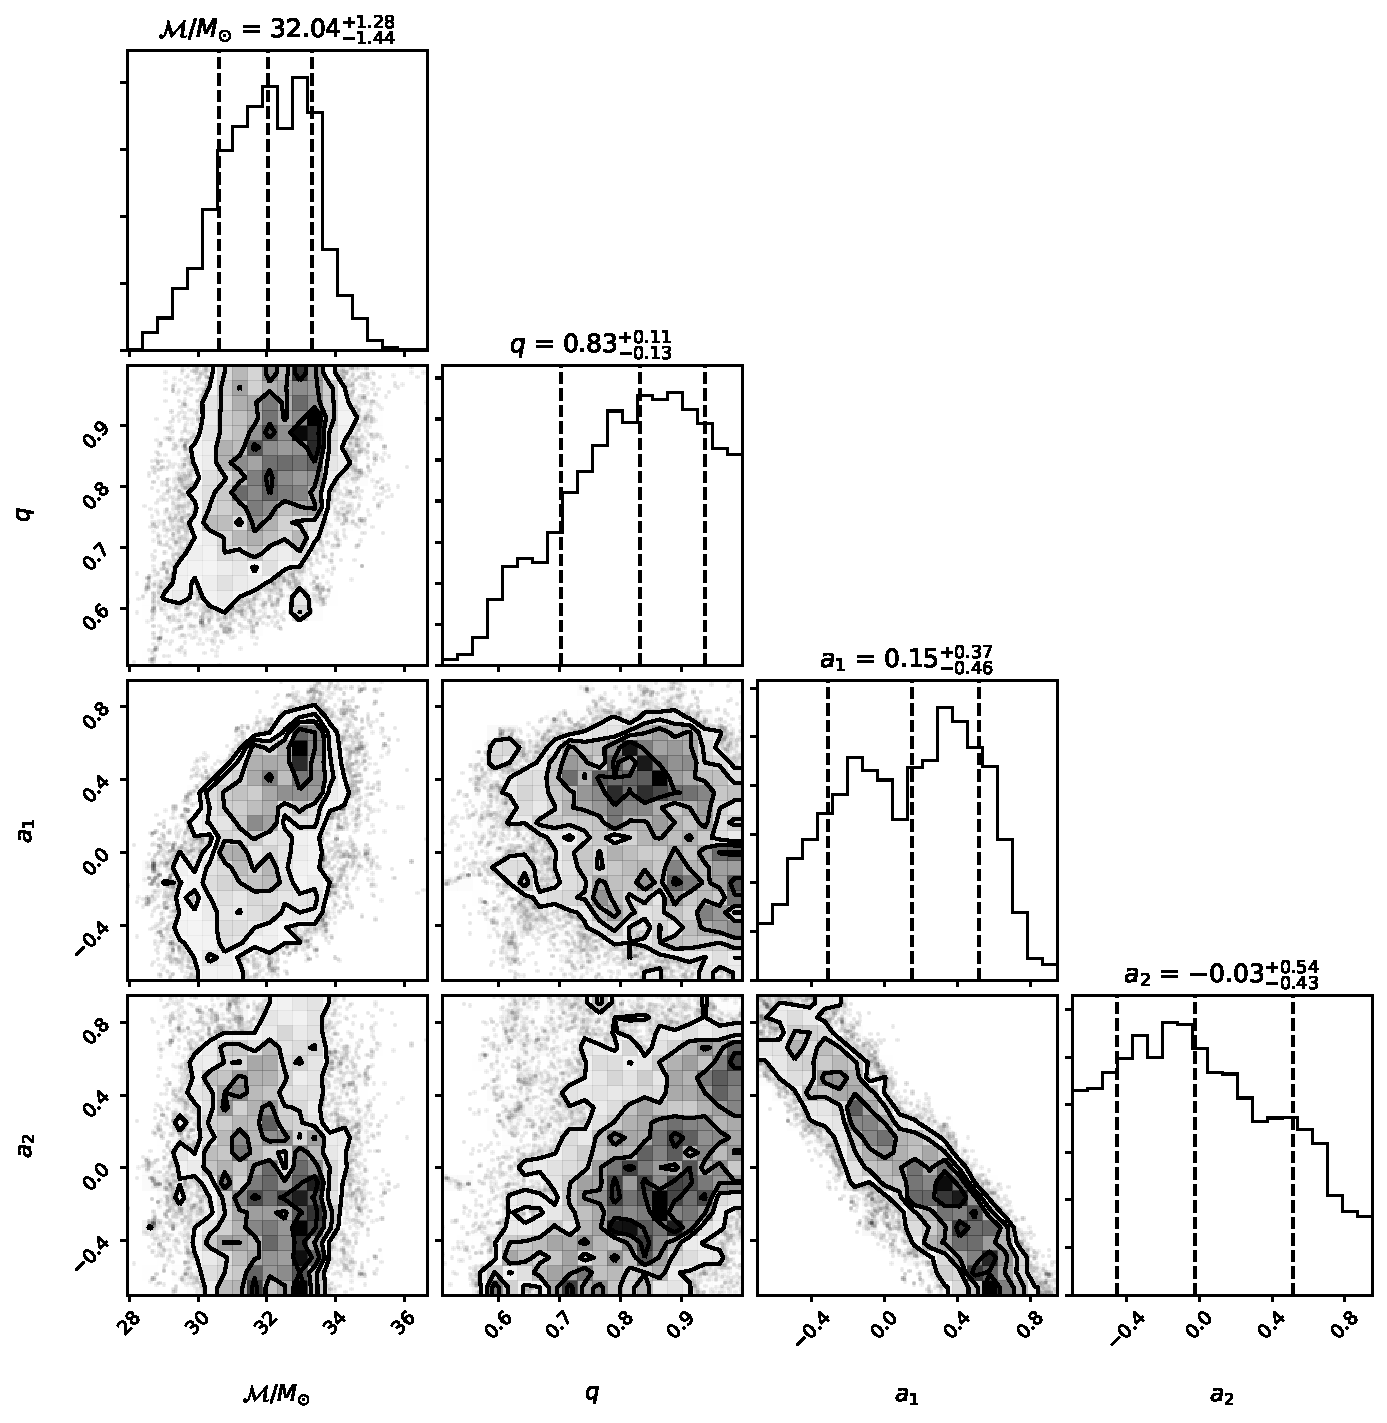
\includegraphics[width=.75\linewidth, trim = {3cm 0cm 3cm 0cm}]{img/intrinsic.pdf}
%	\caption{
%Marginalized posteriors for the chirp mass $\mathcal{M}_c$, inverse mass ration $\bar{q}=\frac{1}{q}$ and spins $s_1, s_2$ for GW150914. We report the histograms for the one dimensional posteriors of each quantity; the dashed lines reports the median value as well as the $68\%$ credible interval.
%In the contour plots, we report the two dimensional posteriors for each pair of quantities.
%The figure holds $16411$ samples and is generated with Python package \texttt{corner} \cite{pycorner}.
%}
%	\label{fig:PDF_BBH}
%\end{figure}
%%%%%%%%%%%%%
%%%%%%%
%\begin{figure}
%	\centering
%    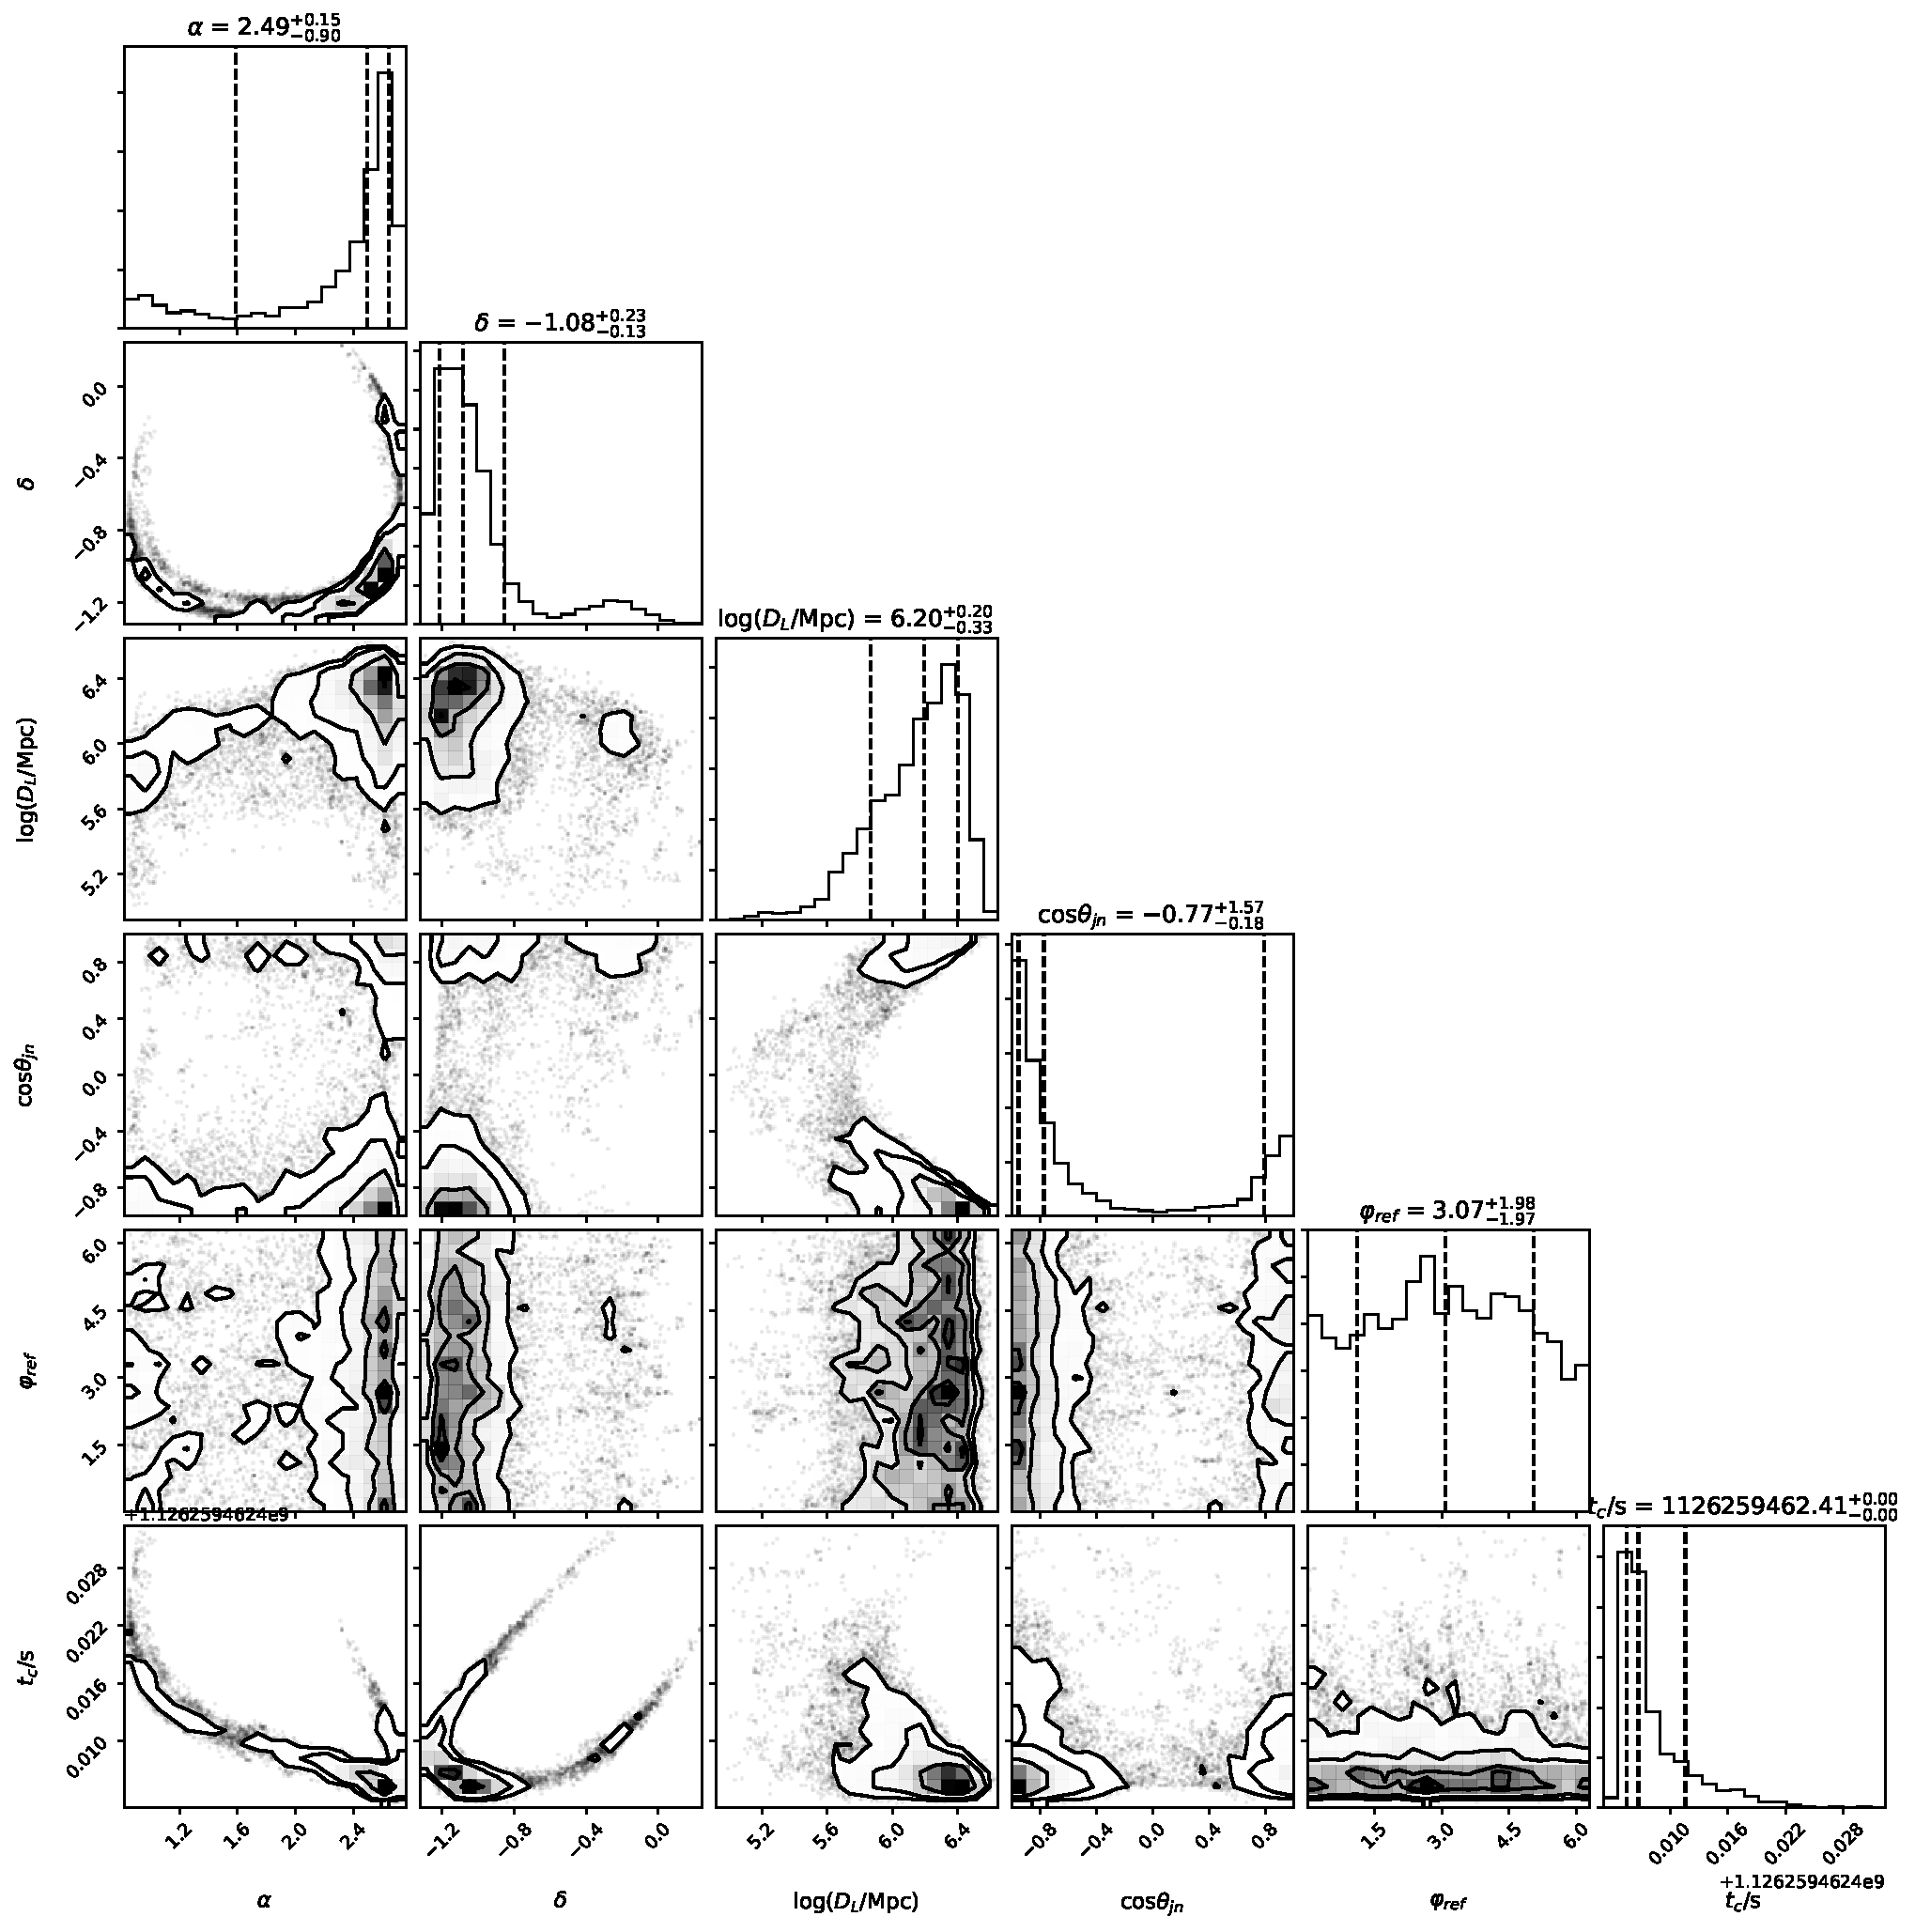
\includegraphics[width=.75\linewidth, trim = {3cm 0cm 3cm 0cm}]{img/extrinsic.pdf}
%	\caption{
%Marginalized posteriors for the sky position angles, luminosity distance, time of coalescence and cosine of the inclination of the orbital plane for GW150914. We report the histograms for the one dimensional posteriors of each quantity; the dashed lines reports the median value as well as the $68\%$ credible interval.
%In the contour plots, we report the two dimensional posteriors for each pair of quantities.
%The figure holds $16411$ samples and is generated with Python package \texttt{corner} \cite{pycorner}.
%}
%	\label{fig:PDF_BBH_extrinsic}
%\end{figure}
%%%%%%%%%%%%%
%We note that the predictions of \texttt{mlgw} are consistent with those of the LIGO-Virgo collaboration.
%The mass related parameters (i.e. chirp mass, total mass and individual masses) are very close to their reference value.
%The same happens for luminosity distance and for the final BH mass and spins.
%\par
%Despite being compatible with the reference values due to high uncertainties, the predicted values for the spins are rather different from the LIGO-Virgo reference values.
%Indeed, the measurement of individual spins are difficult due to spin degeneracy of the waveform, as explained in \cite{Baird2013spin_degeneracy} \cite{Purrer2015meas_spin_deg} with a study of the PN waveform.
%As a consequence, only the effective spin parameter ${\chi_{eff} = \frac{m_1 s_1 + m_2 s_2}{M}}$ can be reliably measured.
%In fact, the two measures of $\chi_{eff}$ agree well with each other: a further confirmation of \texttt{mlgw} accuracy.
%The same feature can be observed on the probability distribution $p(s_1,s_2|\mathcal{D})$ in figure~\ref{fig:PDF_BBH}: individual spins are poor constrained but the ``slope" of their correlation (i.e. the effective spin parameter) is well measured.
%\par
%We note that our model slightly overestimates the value of the BHs masses. This feature was already noted for a PE run with \texttt{TEOBResumS}. The fact that we obtain the same result means that \texttt{mlgw} is able to recover with details the training model.
%\par
%Finally, we see that the two Bayes factors are similar: the Bayesian analysis assigns to both a similar probability that the GW150914 is actually described by the model.
%However, the evidence for \texttt{mlgw} appears to be slightly higher: probably, our priors cover a smaller region than that in the LIGO-Virgo analysis.
%\par



%%%%%%%%%%%%%%%%%%%
\section{Final remarks and future prospects}
We built a ready-to-use Machine Learning model which generates the gravitational wave signal from a binary Black Hole coalescence. The code is released as the package \texttt{mlgw} available via the \texttt{PyPI} Python package repository. 
Our model was built for the case of aligned spins (i.e. the non precessing case) and returns a wave given the BH's masses $m_1, m_2$ and (dimensionless) spins $s_1, s_2$ taking into account the correct dependence on source luminosity distance $d_L$, inclination angle $\iota$ and reference phase $\varphi_0$.
Our model shows excellent agreement with the underlying training set. At test times the median mismatch is $\bar{\mathcal{F}}\sim 5 \cdot 10^{-3}$. Lastly, the generation time from \texttt{mlgw} is smaller than the underlying training model by a factor of $\sim ????$, for a waveform starting at a frequency of $\SI{5}{Hz}$.
\texttt{mlgw} performance matches closely those of a ROM, which is the state-of-the-art for a quick generation.
\par
Remarkably, we discovered that a PCA is able to reproduce a high dimensional wave using a few number of variables. As for the regression model itself, the MoE model, currently it is the ``bottleneck" of the model accuracy. For this reason, we explored several alternative regression methods, including neural networks, but none of them showed better performance.
Note that underfitting may be an issue whenever the training model shows intrinsic noise due to mis-modeling, e.g. relations that are supposed to be continuous are not, or even due to poor numerical integration schemes.
\par
Our work opens up interesting opportunities in GW data analysis.
As shown in fig.~\ref{fig:time_performance_hist}, the model is the most useful whenever a long waveform is required. Furthermore, the waveform generation time does not depend on the complexity of the underlying surrogate model. The training WFs can be computed with high accuracy, also at high computational cost, without affecting the performance of the WF generation.
\par
This fact is crucial for detection of low frequency signals, as is the case for ET. The analysis of such signals can be performed in the same time required to deal with shorter signals: it will become feasible, even with a small amount of resourches, \textit{without any loss of WF quality}.
In \cite{} (\sschmidt{plot in email}), it was shown that training model TEOBResumS matches accurately the numerical relativity WFs, even in the case of ET noise curve is used (see plot in the email). Since our model closely reproduces TEOBResumS, it is likely to achieve the target accuracy for the employment in the ET data analysis.
\sschmidt{Here I wanted to include the plot sent by Nagar. Is it in a paper? Do we include it here? Or do we just skip it??}
\par
As already noted, the fact that a parameter estimation with \texttt{mlgw} is remarkably fast opens up the opportunity for an analysis of the catalog of all the observed GW events.
By training (and the training procedure is moderately quick) \texttt{mlgw} with different surrogate models, it will be possible to compare their predictions on several observed events. This could allow to detect systematic biases or to prefer a model over another by means of Bayesian model selection (i.e. by comparing different model evidences).
A further paper will be devoted to such analysis.
\par
\sschmidt{Is there more to say on that?? E.g. about ROM??}\\
\par
However, our work is far from being over and several issues still require attention.
\par
First of all, the potential speed up of parameter estimation can be even higher, if we take advantage of the closed form expression of the waveform provided by our model.
Indeed, a closed form expression for the WF allows for prompt computation of the gradients with respect to the orbital parameters $ \boldsymbol{\vartheta} = (m_1,m_2, {s}_1,{s}_2) $.
Hamiltonian Montecarlo \cite{betancourt2017hamiltonianMC}~\cite{Porter2014Hamiltonian_MonteCarlo}, a variant of Markov chain Montecarlo, employs gradients of the waveform to perform an effective sampling of the posterior distibution, which is able to ``find quickly" the high density regions.
%Porter and Carré \cite{Porter2014Hamiltonian_MonteCarlo} applied Hamiltonian Montecarlo to parameter estimation. However, they only use analytical waveforms, which completely neglects the late inspiral and the merger.
%Our Machine Learning model could, in principle, extend the application of Hamiltonian Montecarlo to waveform which included also late inspiral, merger and ringdown.
It would provide a state-of-the-art accurate parameter estimation and, at the same time, it will offer a substantial speed up.
We believe that this is a promising option and it is among the natural continuations of our work.
\par
Another option, so far never explored, is to use the gradients of the WF for a fast exploration of the likelihood landscape. With any gradient based optimizer, it should be easy to jump to a \textit{local} maximum of the likelihood. Such information can be used to reliably locate a \textit{global} maximum of the likelihood. Once a global maximum is found, the sampling from the posterior distribution should be quicker to perform, yielding an improvement to the overall analysis.
\par
In our model we did not consider precessing system. We made this choice to keep the problem simple.
The expertise gained for the simple non precessing case can be applied to deal with the complicacies posed by the precessing case.
A good starting point is given in \cite{Schmidt2015Precession}. The dynamics (dependent on 6 parameters) is mapped to a simpler problem, where the precession is controlled by a single parameter. The mapping is as follows:
\begin{align*}
	(s_{1x},s_{1y}, s_{1z}) &\longmapsto (s_{P},0, s_{1z})\\
	(s_{2x},s_{2y}, s_{2z}) &\longmapsto (0, 0, s_{2z})
\end{align*}
where $s_P = s_P(q,s_{1x},s_{1y}, s_{2x},s_{2y})$ (see \cite[eq. 3]{Schmidt2015Precession}).
In the authors' word, the effective spin parameter $s_{P}$ ``accurately captures the dominant precession-induced features in GW signals across the full parameter space".
The waveform dependence on the effective spin parameter $s_P$ can be fitted by a ML model in the same fashion of the other orbital parameters, thus simplyfing the regression problem.
\par
All surrogate models provides numerical solutions to approximate form of the Einstein equations. They are useful to catch the dominant physics but we expect them to show a degree of inaccuracy, especially close to coalescence.
Numerical relativity solves numerically the unapproximated Einstein equations and so far yields the best available solutions.
Clearly, NR waveforms are much slow to generate and cannot be used in parameter estimation.
Our model could be trained on the publicly available NR waveforms catalogs (see e.g. \cite{Mroue2013NRWFcatalog} and \cite{Healy2017NRWFcatalog}) and would provide the best generalization of the numerical waveform.
If the model proved to be reliable and effective, we could dispense with the surrogate models altogether and use only NR inputs for parameter estimation. This would ensure that all the relevant physics close to merger is adequately captured.
Furthermore, a training set of NR waveforms can be used to address problems where an approximation to Einstein equations (such as PN expansion) is not available.
\par
\sschmidt{Are you sure of it??? Probably you should say that you don't know enough on the matter and that you will have to investigate...}\\
Unfortunately, at the moment there are too few NR waveforms ($O(10^2)$) available to perform a reliable training: we need at least $O(10^3)$ waveforms. However, in the future we expect more and more waveforms to be included in the dataset, eventually allowing for a reliable training.
Furthermore, NR waveforms are too short as compared to detected signals in interferometers. Probably, some form of hybridization from PN models is required to tackle the inspiral phase.
\par
Our machine learning approach to signal generation is very flexible and it provides a general framework. We expect it to work for every source for which a number of training waveforms are available (also those for which no surrogate models are available).
Machine learning models for various range of sources can be crucial in the future, where signals from a number of different sources are expected to be detected. In that scenario, a parameter estimation must be able to detect among different source and this will require a lot of computational work. Speed up will be more pressing.












